\documentclass[11pt]{article}
\usepackage[T1]{fontenc}
\usepackage{lmodern}
\usepackage[margin=1.05in]{geometry}
\usepackage{amsmath,amssymb,amsthm,mathtools}
\usepackage{microtype}
\usepackage{booktabs,longtable,array}
\usepackage{tikz}
\usetikzlibrary{arrows.meta,positioning,calc}
\usepackage{listings}
\usepackage[colorlinks=true,linkcolor=blue,citecolor=blue,urlcolor=blue]{hyperref}
\hypersetup{pdftitle={Squarefree values of quartics and power-free values of polynomials},pdfauthor={OpenAI}}
\newtheorem{theorem}{Theorem}[section]
\newtheorem{proposition}[theorem]{Proposition}
\newtheorem{lemma}[theorem]{Lemma}
\newtheorem{corollary}[theorem]{Corollary}
\theoremstyle{definition}
\newtheorem{definition}[theorem]{Definition}
\newtheorem{remark}[theorem]{Remark}
\newtheorem{example}[theorem]{Example}
\newcommand{\Q}{\mathbb Q}
\newcommand{\Z}{\mathbb Z}
\newcommand{\R}{\mathbb R}
\newcommand{\C}{\mathbb C}
\newcommand{\N}{\mathbb N}
\newcommand{\eps}{\varepsilon}
\numberwithin{equation}{section}
\lstset{basicstyle=\ttfamily\footnotesize,columns=fullflexible,keepspaces=true,breaklines=true,frame=single}
\pdfinfoomitdate=1
\pdftrailerid{}
\pdfsuppressptexinfo=15
\title{Squarefree values of quartics and power-free values of polynomials}
\author{OpenAI}
\date{September 24, 2026}
\begin{document}
\maketitle
\begin{abstract}
We prove that every irreducible integer quartic with no fixed prime-square
divisor takes squarefree values with the predicted positive Euler-product
density. More generally, we obtain the corresponding $(d-2)$-power-free
density in degrees $4\le d\le8$. The proof combines number-field factorization,
determinant estimates with adaptive auxiliary primes, and explicit
low-degree geometry. Together with Browning's theorem for higher degrees,
this gives the $(d-2)$-power-free density for every $d\ge4$.
\end{abstract}
\tableofcontents
\section{Introduction}
\label{sec:introduction}

For an integer $k\ge2$, an integer $a$ is \emph{$k$-power-free} if no prime
power $p^k$ divides $a$. This convention includes negative integers and
excludes zero. Given $f\in\Z[x]$, write
\[
 \rho_f(q)=\#\{a\in\Z/q\Z:f(a)\equiv0\pmod q\},\qquad
 S_{f,k}(X)=\#\{1\le n\le X:f(n)\text{ is $k$-power-free}\}.
\]
The necessary local condition is
\begin{equation}
 \rho_f(p^k)<p^k\quad\text{for every prime }p.
 \label{eq:local-admissibility}
\end{equation}
It says that no prime $k$th power divides every value of $f$. The natural
candidate for the density is the product of the proportions that survive
these separate congruence conditions.

\begin{theorem}\label{thm:density}
Let $f\in\Z[x]$ be irreducible over $\Q$, of degree $d$ with
$4\le d\le8$, and put $k=d-2$. If \eqref{eq:local-admissibility} holds,
then
\[
 S_{f,k}(X)=c_{f,k}X+o_f(X),\qquad
 c_{f,k}=\prod_p\left(1-\frac{\rho_f(p^k)}{p^k}\right)>0.
\]
No primitivity or sign condition on the leading coefficient is required.
\end{theorem}

For quartics this is a squarefree-value density theorem. In degrees
$5,6,7,8$, the respective excluded powers are $3,4,5,6$.
The statement concerns positive integer inputs and imposes no bound on
the height of the fixed polynomial's coefficients. The error term is not
asserted to be uniform as $f$ varies.

In particular, the quartics $x^4+2$ and $x^4+1$ have positive squarefree-value
density. The first is Eisenstein at $2$; the second is the eighth cyclotomic
polynomial. For $x^4+2$, its value at zero excludes a fixed odd prime square,
and its value at one excludes a fixed square of $2$. The value at zero
of $x^4+1$ is one, so its local condition is immediate.

\subsection{Earlier results and the higher-degree consequence}

The power-free-value problem has a long history. Ricci obtained
the asymptotic in the range $k\ge d$ \cite{Ricci1933}.
For $d\ge3$, Erd\H{o}s proved infinitude for exponent $d-1$, and Hooley obtained
the corresponding asymptotic \cite{Erdos1953,Hooley1967}; see also
the historical discussion in \cite[Introduction]{HeathBrown2013Powerfree}.
The cubic squarefree case therefore belongs to this classical range.
Already in 1953, Erd\H{o}s singled out the unresolved squarefreeness
of $n^4+2$ \cite[p.~425]{Erdos1953}. In his 1965 survey he returned
to this example when describing the obstacle at exponent $d-2$
\cite[Section~6, p.~219]{Erdos1965}.

Nair obtained the asymptotic for
$k\ge(\sqrt2-\tfrac12)d$ \cite{Nair1976}, with further developments
by Nair and Huxley--Nair \cite{Nair1979,HuxleyNair1980}.
The 1976 bound reaches $k=d-2$ for $d\ge24$.
Heath-Brown's affine determinant method gave the range
$k\ge(3d+2)/4$ \cite[Theorem~16]{HeathBrown2006Counting}, reaching
$k=d-2$ for $d\ge10$. Combining that method with Salberger's
global determinant estimates, Browning improved the range to
$k\ge(3d+1)/4$ \cite{Browning2011PowerFree}, which reaches
$k=d-2$ for $d\ge9$.
We use the formulation and published reproof in
Xiao \cite[Theorem~9.1 and Section~9]{Xiao2017PowerFree}:
the input interval is $1\le n\le X$ and the constant is the
Euler product over all residue classes modulo $p^k$.

The shape of the polynomial can permit stronger estimates.
Heath-Brown proved an asymptotic with a power-saving error for
irreducible binomials $x^d+c$ when $k\ge(5d+3)/9$
\cite[Theorem~1]{HeathBrown2013Powerfree}. At $k=d-2$ this covers
such binomials in degrees $d\ge6$, while imposing the special
binomial form. Reuss obtained a power-saving error for the general
degree-$d$ polynomial at exponent $d-1$
\cite[Theorem~2]{Reuss2015PowerFree}. The quartic theorem above
concerns squarefree values at positive integer arguments for each
fixed admissible polynomial.

Other important directions involve different hypotheses or
quantifiers. Granville showed that the $abc$ conjecture yields
the predicted squarefree-value density for separable integer
polynomials with no fixed prime-square divisor
\cite[Theorem~1]{granville1998abc}.
Greaves and Helfgott studied squarefree values of binary forms;
Helfgott's Theorems~5.1--5.2 distinguish univariate cubics from
homogeneous forms in two variables of degree at most six
\cite{Greaves1992,Helfgott2004}. A density in two integer variables
does not by itself give the density on the fixed line with second
coordinate one. Recent results of Browning--Shparlinski and Sofos
study the discrepancy from the predicted squarefree count on
average over polynomial coefficient families
\cite[Theorems~1.1--1.2]{BrowningShparlinski2024},
\cite[Theorem~1.1]{Sofos2026}; those averaged statements
do not imply a theorem for every fixed polynomial.

Carella's preprint claims squarefree-value asymptotics for both
$n^4+1$ and $n^4+2$ \cite[Theorems~1.1--1.2]{carella2023squarefree}.
Zapata Ceballos--Jalalvand claim positive density for monic
irreducible degree-$2q$ polynomials with squarefree fixed divisor
whose root field contains a degree-$q$ Galois subfield, where $q$
is prime; this includes $n^4+1$
\cite[Theorem~1.1]{zapataceballosjalalvand2026squarefree}.
We do not use either claim as a
theorem input. Our large-prime estimate and sieve transfer are
proved independently below.

The new argument in this paper concerns degrees four through eight.
For higher degrees, Browning's theorem supplies a direct consequence.

\begin{corollary}\label{cor:all-degrees}
Let $f\in\Z[x]$ be irreducible over $\Q$ of degree $d\ge4$, and
put $k=d-2$. If $f$ has no fixed prime $k$th-power divisor, then
\[
 S_{f,k}(X)=c_{f,k}X+o_f(X),\qquad
 c_{f,k}=\prod_p\left(1-\frac{\rho_f(p^k)}{p^k}\right)>0.
\]
\end{corollary}

\begin{proof}
For $4\le d\le8$ use Theorem~\ref{thm:density}. For $d\ge9$,
\[
 d-2\ge\frac{3d+1}{4},
\]
so Browning's theorem, in the cited form of Xiao, applies to the
primitive positive-leading part of $f$. Lemma~\ref{lem:density-content}
transfers its density to $f$, retaining the original local factors.
\end{proof}

The factorwise large-prime estimates also give a fixed-product
consequence. Here a nonzero polynomial is \emph{separable over $\Q$}
if each of its nonconstant irreducible factors occurs with multiplicity one.

\begin{corollary}[Separable products and simultaneous values]
\label{cor:separable-products}
Fix an integer $k\ge2$. Let $F\in\Z[x]\setminus\{0\}$ be separable over
$\Q$, with every nonconstant irreducible factor of degree at most $k+2$.
If $\rho_F(p^k)<p^k$ for every prime $p$, then
\[
 S_{F,k}(N)=c_{F,k}N+o_{F,k}(N),\qquad
 c_{F,k}=\prod_p\left(1-\frac{\rho_F(p^k)}{p^k}\right)>0.
\]
More generally, let $\mathbf F=(F_1,\ldots,F_r)$, with $r\ge1$, be a fixed
family of nonzero integer polynomials, each separable over $\Q$ with all
nonconstant irreducible factors of degree at most $k+2$. Factors may be
shared by different $F_i$. Put
\[
 \Omega_p=\{a\in\Z/p^k\Z:p^k\mid F_i(a)\text{ for at least one }i\}.
\]
Let $S_{\mathbf F,k}(N)$ count the integers $1\le n\le N$ for which every
$F_i(n)$ is $k$-power-free. If $\#\Omega_p<p^k$ for every prime $p$, then
\[
 S_{\mathbf F,k}(N)=c_{\mathbf F,k}N+o_{\mathbf F,k}(N),\qquad
 c_{\mathbf F,k}=\prod_p\left(1-\frac{\#\Omega_p}{p^k}\right)>0.
\]
\end{corollary}

The first assertion requires the value of the entire product $F$ to be
$k$-power-free. The second imposes power-freeness separately on the
$F_i(n)$, not on their product, and uses the joint local condition
$\Omega_p$ rather than a product of individual local factors.
All polynomials, their number, and $k$ are fixed; no uniform or
power-saving error is asserted here. The proof is at the end of
Section~\ref{sec:sieve}.

Our method combines number-field factorization with approximating
determinants, following the framework developed by Reuss for
power-free polynomial values \cite[Sections~3--6]{Reuss2015PowerFree}.
Heath-Brown's determinant arguments for
squarefree values of $n^2+1$ and for power-free binomial values
provide related precedents
\cite{HeathBrown2012Squarefree,HeathBrown2013Powerfree}.
The real determinant method originates in work of Bombieri--Pila;
Heath-Brown developed the prime-adic and approximating forms used
in this line of arguments, and Salberger developed their local
Hilbert and global congruence aspects
\cite{BombieriPila1989,HeathBrown2002Density,HeathBrown2009Sums,
Salberger2007,Salberger2023}.
The uniform affine counting theorem, the explicit weighted Hilbert
calculations and the quartic surface and curve arguments needed here
are proved below.

\subsection{The large-prime problem}

The finite-prime part of the problem follows from the Chinese remainder
theorem. For primes outside a fixed finite set, separability and Hensel
lifting give $\rho_f(p^k)\le d$. Consequently, for fixed large $Y$, primes
$Y<p\le X$ remove at most
\[
 O_f\bigl(XY^{1-k}+\pi(X)\bigr)
\]
integers in $(X,2X]$. The remaining task is to control primes larger than
the length of the input interval. We prove the following estimate.

\begin{proposition}\label{prop:large-prime-tail}
Let $f\in\Z[x]$ be primitive and irreducible, with positive leading
coefficient and degree $4\le d\le8$. Put $k=d-2$. There exists
$\delta=\delta_f>0$ such that
\[
 \#\{n\in\Z:X<n\le2X,\ p^k\mid f(n)
          \text{ for some prime }p>X\}
 \ll_f X^{1-\delta}.
\]
\end{proposition}

The proposition does not require local admissibility. In
Section~\ref{sec:sieve}, we prove explicitly that it implies
Theorem~\ref{thm:density}, including the stated sign and content
generality. The density argument first holds the finite-prime cutoff
fixed while $X$ tends to infinity, and then lets the cutoff tend to
infinity. This order gives the exact Euler product without an assertion
of a power-saving error in the density asymptotic.

\subsection{Proof strategy}

Fix a dyadic prime interval $P\le p\le2P$, and choose one such prime
for each input being counted. Write $P=X^\eta$ and $b=d-k\eta$.
The elementary relation $f(n)=yp^k$ puts the chosen triples on the
surface $f(x)=yz^k$, with coordinate sizes $X,X^b,X^\eta$.
A weighted determinant argument on this surface suffices when $\eta$
is large. The harder range requires more information from the
factorization of $f$.

Let $\theta$ be a root of $f$ and let $K=\Q(\theta)$. Ideal
factorization and the unit theorem produce integral elements
$\alpha,\beta\in K$ satisfying
\[
 \alpha^k\beta=\mu(n-\theta)
\]
for a fixed nonzero integer $\mu$. Their conjugates are balanced:
the sizes of $\alpha$ and $\beta$ at each embedding are respectively
comparable to $P^{1/d}$ and $X^{b/d}$. Integer coordinates in a fixed
integral basis therefore give two boxes, while their projective
directions satisfy explicit polynomial equations. Near a balanced
point, and after choosing one of finitely many local branches, either
direction determines the other analytically once $1/n$ is specified.

We partition these directions into small paired boxes. An
archimedean determinant gives a polynomial equation on the points
in each pair. Components defined by an equation in only one of the
two coordinate groups receive a second cut. Explicit complete
intersection calculations measure the independent monomials available
on the resulting sets. The distinction between a mixed equation and a
pure equation is important: the latter also reduces the number of
independent Taylor monomials in the local determinant.

Two further steps turn these cuts into a count. First, a reduced basis
of the integer lattice associated with a direction box makes its
points smaller in new integral coordinates. An exceptionally short
lattice vector also limits the number of boxes in which it can occur.
Second, we apply the general affine counting theorem proved in
Section~\ref{sec:affine-counting}, using lower bounds
for weighted spaces of polynomial functions. Its proof repeatedly
uses residue classes at small auxiliary primes. Its auxiliary
varieties depend on earlier choices of primes; a random deletion
argument controls the primes at which their equations fail to give
smooth local coordinates. This permits a uniform count through
successive dimension drops.

For quartics, surfaces and curves need sharper geometric bounds.
On a surface, the difficult projections have degree one or two.
The quadric case supplies an additional field degree. On a plane,
a deficient bound would force either a polynomial of degree at most
four on a general line or a degree-two rational map on the line of
directions to have four distinct critical values. On a curve, the limiting
case is a polynomial of degree five with four prescribed critical
values. Up to a normalization of two critical points, only finitely
many such polynomials occur. Their integer values in the input interval
form one set of size $O_f(X^{1/5})$, which is removed once before summing
over boxes. The remaining curve estimates and an exact finite choice
of parameters give a common power saving.

\subsection{Organization}

Figure~\ref{fig:proof-flow} shows how the principal estimates feed
into the density theorem. Its arrows indicate uses of established
modules; the order of the sections places the uniform counting
statement before its arithmetic applications.

\begin{figure}[ht]
\centering
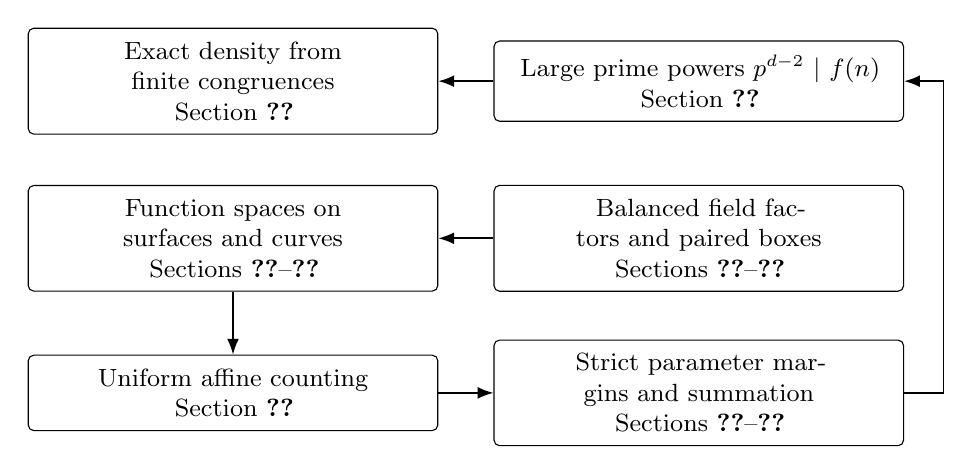
\begin{tikzpicture}[
  node distance=8mm and 7mm,
  flowbox/.style={draw,rounded corners=2pt,align=center,text width=0.40\textwidth,
    inner sep=5pt,font=\small},
  arrow/.style={-{Latex[length=2mm]},semithick}]
\node[flowbox] (sieve) {Exact density from finite congruences\\
  Section~\ref{sec:sieve}};
\node[flowbox,right=of sieve] (tail) {Large prime powers $p^{d-2}\mid f(n)$\\
  Section~\ref{sec:tail-proof}};
\node[flowbox,below=of tail] (boxes) {Balanced field factors and paired boxes\\
  Sections~\ref{sec:arithmetic-boxes}--\ref{sec:lattice-boxes}};
\node[flowbox,left=of boxes] (hilbert) {Function spaces on surfaces and curves\\
  Sections~\ref{sec:hilbert-bounds}--\ref{sec:curves}};
\node[flowbox,below=of hilbert] (count) {Uniform affine counting\\
  Section~\ref{sec:affine-counting}};
\node[flowbox,right=of count] (parameters) {Strict parameter margins and summation\\
  Sections~\ref{sec:parameters}--\ref{sec:tail-proof}};
\draw[arrow] (boxes) -- (hilbert);
\draw[arrow] (hilbert) -- (count);
\draw[arrow] (count) -- (parameters);
\draw[arrow] (parameters.east) -- ++(5mm,0) |- (tail.east);
\draw[arrow] (tail) -- (sieve);
\end{tikzpicture}

\caption{The number-field route to the large-prime bound and the
exact density. The direct-surface estimate handles the complementary
upper prime range in Section~\ref{sec:tail-proof}.}
\label{fig:proof-flow}
\end{figure}

Section~\ref{sec:sieve} gives the density reduction, and
Section~\ref{sec:affine-counting} proves the general counting theorem.
Sections~\ref{sec:arithmetic-boxes}--\ref{sec:lattice-boxes} construct
the number-field boxes, determinant cuts and lattice coordinates.
Section~\ref{sec:hilbert-bounds} establishes weighted Hilbert bounds;
Sections~\ref{sec:quartic-geometry} and~\ref{sec:curves} sharpen them
for quartic surfaces and curves. Section~\ref{sec:parameters} selects
the parameters, and Section~\ref{sec:tail-proof} proves the
large-prime estimate and completes the density theorem.
Section~\ref{sec:cyclotomic} gives the explicit cyclotomic density,
retains a quantitative central-prime estimate, and explains the
special factorization, level equation and Pell alternative.

\section{From a large-prime tail to the exact density}
\label{sec:sieve}

The geometric argument will estimate large prime-power divisors for a
primitive polynomial with positive leading coefficient. We first prove
that this is enough for the full density statement. The finite-prime
conditions must still be imposed on the original polynomial: removing
its content can change the corresponding factors of the Euler product.

\begin{proposition}[Sieve transfer]\label{prop:sieve-transfer}
Let $f\in\Z[x]$ be irreducible over $\Q$, of degree $d\ge2$, and let
$k\ge2$. Suppose that $\rho_f(p^k)<p^k$ for every prime $p$.
Write
\[
 f=s c g,\qquad s\in\{-1,1\},\quad c\in\N,
\]
where $c$ is the positive content of $f$ and $g\in\Z[x]$ is primitive
with positive leading coefficient. Assume that
\begin{equation}
 T_g(X):=\#\{n\in\Z:X<n\le2X,\ p^k\mid g(n)
                 \text{ for some prime }p>X\}=o_{g,k}(X).
 \label{eq:sieve-tail-hypothesis}
\end{equation}
Then
\[
 S_{f,k}(N)=c_{f,k}N+o_{f,k}(N),\qquad
 c_{f,k}=\prod_p\left(1-\frac{\rho_f(p^k)}{p^k}\right)>0.
\]
\end{proposition}

\begin{proof}
\emph{Normalization and local factors.}
Multiplication by $s$ does not affect divisibility. The polynomial $g$
is irreducible over $\Q$, and it inherits local admissibility from $f$.
Neither polynomial has an integer root, because its degree is at least
two. Thus none of the counted values is zero.

For a prime $p\mid c$, put $e=v_p(c)$. Local admissibility forces $e<k$,
and
\begin{equation}
 \rho_f(p^k)=p^e\rho_g(p^{k-e}),\qquad
 1-\frac{\rho_f(p^k)}{p^k}
 =1-\frac{\rho_g(p^{k-e})}{p^{k-e}}.
 \label{eq:sieve-content-factor}
\end{equation}
Indeed, $p^k\mid f(a)$ is equivalent to $p^{k-e}\mid g(a)$, and each
class modulo $p^{k-e}$ has exactly $p^e$ lifts modulo $p^k$.
For $p\nmid c$ the root counts of $f$ and $g$ modulo $p^k$ agree.
Once $X$ exceeds every prime divisor of $c$, the large-prime exceptional
sets for $f$ and $g$ are therefore identical.

Let $\mathcal B$ contain the prime divisors of $c$, the leading coefficient
of $g$, and the discriminant of $g$. This is a finite set. If
$p\notin\mathcal B$, reduction of $g$ has degree $d$ and simple roots.
Each root modulo $p^j$ lifts uniquely modulo $p^{j+1}$: the expansion
\[
 g(a+p^j u)\equiv g(a)+p^j u g'(a)\pmod{p^{j+1}}
\]
determines $u$ modulo $p$, since $g'(a)$ is invertible there. Consequently
\begin{equation}
 \rho_f(p^k)=\rho_g(p^k)=\rho_g(p)\le d
 \qquad(p\notin\mathcal B).
 \label{eq:sieve-root-bound}
\end{equation}

Put $q_p=\rho_f(p^k)/p^k$. Each $q_p<1$ by hypothesis, and
\eqref{eq:sieve-root-bound} gives $\sum_p q_p<\infty$ because $k\ge2$.
For all sufficiently large $p$, $q_p\le1/2$ and
$-2q_p\le\log(1-q_p)\le-q_p$. Thus the Euler product converges to a
strictly positive number. Its finitely many factors at primes in
$\mathcal B$ are retained exactly, including
\eqref{eq:sieve-content-factor}.

\emph{The finite sieve and the intermediate primes.}
Fix an integer $Y\ge2$ exceeding every prime in $\mathcal B$, and set
\[
 Q_Y=\prod_{p\le Y}p^k,\qquad
 c_Y=\prod_{p\le Y}\left(1-\frac{\rho_f(p^k)}{p^k}\right).
\]
Let $A_Y(X)$ count the integers $n\in(X,2X]$ for which
$p^k\nmid f(n)$ for every $p\le Y$. The Chinese remainder theorem gives
exactly $Q_Yc_Y$ permitted classes modulo $Q_Y$. Counting each class in
the interval gives
\begin{equation}
 A_Y(X)=c_YX+O(Q_Y).
 \label{eq:sieve-finite-crt}
\end{equation}
Here $Y$ remains fixed as $X$ tends to infinity.

Write $A(X)$ for the count of all $k$-power-free values in $(X,2X]$.
For $X>Y$, the integers removed by primes $Y<p\le X$ number at most
\begin{align}
 I_Y(X)
 &\le\sum_{Y<p\le X}\rho_f(p^k)
                    \left(\frac{X}{p^k}+1\right)\notag\\
 &\le dX\sum_{m>Y}\frac1{m^k}+d\pi(X)
 \le\frac{d}{k-1}XY^{1-k}+d\pi(X).
 \label{eq:sieve-intermediate}
\end{align}
The elementary bound $\pi(X)\ll X/\log X$ is sufficient here.
For all sufficiently large $X$, the remaining exceptional set is counted
by $T_g(X)$, so
\begin{equation}
 0\le A_Y(X)-A(X)\le I_Y(X)+T_g(X).
 \label{eq:sieve-sandwich}
\end{equation}

We can now identify the density. Divide
\eqref{eq:sieve-finite-crt}--\eqref{eq:sieve-sandwich} by $X$ and first
let $X\to\infty$ with $Y$ fixed. The tail hypothesis gives
\[
 c_Y-\frac{d}{k-1}Y^{1-k}
 \le\liminf_{X\to\infty}\frac{A(X)}X
 \le\limsup_{X\to\infty}\frac{A(X)}X
 \le c_Y.
\]
Then let $Y\to\infty$. Since $c_Y\to c_{f,k}$, this proves
\begin{equation}
 A(X)=c_{f,k}X+o_{f,k}(X).
 \label{eq:sieve-dyadic-density}
\end{equation}

\emph{From dyadic intervals to positive inputs.}
Fix an integer $J\ge1$. Apply \eqref{eq:sieve-dyadic-density} to the
finitely many disjoint intervals
\[
 (N/2^{j+1},N/2^j],\qquad 0\le j<J.
\]
For fixed $J$, their total count is
$c_{f,k}N(1-2^{-J})+o_{f,k,J}(N)$. The interval $[1,N/2^J]$ contains
at most $N/2^J$ integers. Hence
\[
 \begin{split}
 c_{f,k}(1-2^{-J})
 &\le\liminf_{N\to\infty}\frac{S_{f,k}(N)}N\\
 &\le\limsup_{N\to\infty}\frac{S_{f,k}(N)}N
 \le c_{f,k}(1-2^{-J})+2^{-J}.
 \end{split}
\]
Letting $J\to\infty$ proves the proposition.
\end{proof}

\begin{remark}\label{rem:sieve-congruences}
A large-prime bound remains valid after imposing any fixed finite
congruence restrictions on $n$, since the restricted exceptional set is
a subset of the unrestricted one. In the finite sieve those restrictions
are combined with the conditions modulo $p^k$ using their least common
multiple as modulus. No independence of overlapping congruence conditions
is needed. In particular, the exact conditions at content primes can be
retained while using the large-prime bound for the primitive polynomial.
\end{remark}

The same normalization also applies when a density theorem for the
primitive polynomial is already available. It does not require a
separate estimate for values in arithmetic progressions.

\begin{lemma}[Removing sign and content]\label{lem:density-content}
Let $f\in\Z[x]$ be irreducible over $\Q$, of degree at least two, and let
$k\ge2$. Suppose that $\rho_f(p^k)<p^k$ for every prime $p$, and write
$f=s c g$, where $s\in\{-1,1\}$, $c$ is the positive content, and $g$ is
primitive with positive leading coefficient. If
\[
 S_{g,k}(N)=c_{g,k}N+o_{g,k}(N),\qquad
 c_{g,k}=\prod_p\left(1-\frac{\rho_g(p^k)}{p^k}\right),
\]
then $S_{f,k}(N)=c_{f,k}N+o_{f,k}(N)$ with the Euler product $c_{f,k}>0$
of Proposition~\ref{prop:sieve-transfer}.
\end{lemma}

\begin{proof}
The normalization and product-convergence arguments above do not use
the tail hypothesis. Thus both Euler products converge, and their
factors are related by \eqref{eq:sieve-content-factor}.
Fix an integer $Y$ exceeding every prime divisor of $c$. For $h=f,g$,
let $B_{h,Y}(N)$ count the integers $1\le n\le N$ avoiding $p^k\mid h(n)$
for every $p\le Y$, and put
\[
 c_{h,Y}=\prod_{p\le Y}\left(1-\frac{\rho_h(p^k)}{p^k}\right).
\]
The finite Chinese remainder calculation gives
$B_{h,Y}(N)=c_{h,Y}N+O(Q_Y)$, with $Q_Y=\prod_{p\le Y}p^k$.

An input counted by $B_{f,Y}(N)-S_{f,k}(N)$ avoids all the small-prime
conditions for $f$ but has a divisor $p^k$ with $p>Y$.
It also avoids the small-prime conditions for $g$, and $p\nmid c$ implies
$p^k\mid g(n)$. Consequently
\[
 0\le B_{f,Y}(N)-S_{f,k}(N)
 \le B_{g,Y}(N)-S_{g,k}(N).
\]
For fixed $Y$, divide by $N$ and let $N\to\infty$. The assumed density
of $g$ yields
\[
 c_{f,Y}-(c_{g,Y}-c_{g,k})
 \le\liminf_{N\to\infty}\frac{S_{f,k}(N)}N
 \le\limsup_{N\to\infty}\frac{S_{f,k}(N)}N
 \le c_{f,Y}.
\]
Letting $Y\to\infty$ proves the claim.
\end{proof}

\begin{proof}[Proof of Corollary~\ref{cor:separable-products}]
Write
\[
 F_i=c_i\prod_{g\in\mathcal G_i}g,\qquad c_i\in\Z\setminus\{0\},
\]
where $\mathcal G_i$ is a set of distinct primitive irreducible polynomials
with positive leading coefficients. Let $\mathcal G=\bigcup_i\mathcal G_i$,
so shared factors are included only once. The joint local condition implies
local admissibility of each $F_i$, and hence of every $g\in\mathcal G$.
For such a factor of degree $d\le k+2$, let $T_{g,k}(X)$ count the integers
$X<n\le2X$ for which $p^k\mid g(n)$ for some prime $p>X$. We first record
\begin{equation}
 T_{g,k}(X)=o_{g,k}(X).
 \label{eq:factorwise-tail}
\end{equation}

For $d\le k$, omit the finitely many integer roots of $g$ and use
$|g(n)|\ll_g X^d$. If $d<k$, the tail is empty for large $X$. If $d=k$,
only primes $X<p\le C_gX$ can occur, for a fixed $C_g$. Outside finitely
many primes, each has at most $d$ roots modulo $p^k$, and an interval of
length $X<p^k$ contains at most one representative of each root. Thus
$T_{g,k}(X)\ll_g\pi(C_gX)=o_g(X)$.
If $d=k+1$, the unweighted triple estimates of Reuss
\cite[Lemma~3 and its proof, and Section~6]{Reuss2015PowerFree} give
$o_g(X)$ triples with $X<n\le2X$, $a>X^{1-\delta}$, $\mu^2(a)=1$, and
$a^{d-1}b=g(n)$, for a suitable fixed $\delta>0$. For large $X$ the
values $g(n)$ here are positive, so $a=p$ and $b=g(n)/p^k$ include every
input counted by $T_{g,k}(X)$.
If $d=k+2\le8$, use Proposition~\ref{prop:large-prime-tail}.
Finally, if $d=k+2\ge9$, then $k=d-2\ge(3d+1)/4$ and $k/d>3/4$.
Xiao's estimate in \cite[Section~9]{Xiao2017PowerFree} is
$E_B(B^{1-\delta})=o_g(B)$ for some fixed $\delta>0$, where
\[
 E_B(\xi)=\#\{1\le n\le B:\ b^k\mid g(n)
                 \text{ for some squarefree integer }b>\xi\}.
\]
Take $B=2X$: eventually $p>X>(2X)^{1-\delta}$, so this exceptional set
contains the tail. This proves \eqref{eq:factorwise-tail} in every case.

Let $\mathcal B$ contain the prime divisors of all $c_i$, leading
coefficients and discriminants of the $g\in\mathcal G$, and resultants
of distinct pairs in $\mathcal G$. This set is finite: all the
discriminants and pairwise resultants are nonzero. For $p\notin\mathcal B$,
no two distinct factors vanish at the same residue modulo $p$, and their
roots are simple. Consequently
\[
 \begin{aligned}
 p^k\mid F_i(n)&\ \Longleftrightarrow\
 p^k\mid g(n)\text{ for some }g\in\mathcal G_i,\\
 \#\Omega_p&\le\sum_{g\in\mathcal G}\rho_g(p^k)
 =\sum_{g\in\mathcal G}\rho_g(p)\le D,
 \end{aligned}
\]
where $D=\sum_{g\in\mathcal G}\deg g$. Once $X$ exceeds all primes in
$\mathcal B$, the large-prime exceptional set for the family is contained
in the union of the sets counted by the $T_{g,k}(X)$, and hence has size
$o_{\mathbf F,k}(X)$.

For fixed $Y$ beyond $\mathcal B$, the Chinese remainder theorem leaves
exactly
\[
 Q_Y\prod_{p\le Y}\left(1-\frac{\#\Omega_p}{p^k}\right)
 \quad\text{classes modulo }Q_Y=\prod_{p\le Y}p^k.
\]
The estimate \eqref{eq:sieve-intermediate}, with $D$ in place of $d$,
bounds the contribution of $Y<p\le X$. Combining it with the family
tail and taking the two limits as in
\eqref{eq:sieve-finite-crt}--\eqref{eq:sieve-dyadic-density} gives the
stated density on positive inputs. The product is positive because its
local factors are positive and $\sum_p\#\Omega_p/p^k<\infty$.
At primes in $\mathcal B$ the full set $\Omega_p$ is retained: in
particular, valuations contributed by different factors of one $F_i$
are not separated there. Taking $r=1$ gives the first assertion with
$\#\Omega_p=\rho_F(p^k)$. Empty products cover nonzero constants, and
the finitely many integer zeros of nonconstant polynomials have no
effect on the asymptotic.
\end{proof}

\section{Affine counting with adaptive auxiliary primes}
\label{sec:affine-counting}

The geometric arguments below place the points to be counted on varieties
whose equations vary with the box.  We first prove a counting theorem
that is uniform for these moving varieties.  Its input is a lower bound
for the number of independent monomials on each subvariety.  Its proof
successively cuts residue classes by polynomial equations.  A deletion
argument controls the primes at which these newly constructed equations
have singular reduction.
The local prime-adic determinant principle is due to Heath-Brown
\cite[Section~3, Lemmas~5--6]{HeathBrown2002Density}; the ordered local Hilbert
and divisibility estimates are developed in
\cite[Lemmas~2.3--2.5]{Salberger2007}. Simultaneous prime
conditions appear in \cite[Theorem~3.2]{Salberger2007} and
\cite[Section~2, Theorem~2.2]{Salberger2023}.
The argument here includes
the additional patch construction and deletion estimate needed when
later varieties depend on earlier prime choices.

Throughout this section, degree means the ordinary degree of projective
closure; for a reducible algebraic set we use the sum of the degrees of
its irreducible components.  Irreducibility is over $\C$.  We use the
degree bounds for intersections and linear projections supplied by
B\'ezout's theorem.  The ambient dimension is fixed.

Fix positive weights $\omega_1,\ldots,\omega_N$.  The weight of the
coordinate monomial $z^\alpha$ is $\omega\cdot\alpha$.  For an affine
algebraic set $A\subseteq\C^N$, define
\[
 H_A(T)=\dim_{\C}\operatorname{span}
 \{z^\alpha|_A:\omega\cdot\alpha\le T\}.
\]
Thus $H_A(T)$ measures the supply of independent polynomial functions
whose sizes in the weighted box are at most a constant times $X^T$.

\begin{theorem}\label{thm:affine-counting}
Fix integers $1\le r\le N$, a degree bound $e_0$, a constant $C$, positive coordinate
weights $\omega_l$, and positive numbers $\delta_1,\ldots,\delta_r$.
For $X\ge2$, let $S\subseteq\Z^N$ satisfy
\[
 |z_l|\le C X^{\omega_l}\quad(z\in S),
\]
and suppose $S$ lies on an algebraic set $Z$ of degree at most $e_0$
and dimension at most $r$.  Assume the following uniform alternative.
For every fixed degree bound $e$, each irreducible subvariety
$A\subseteq Z$ defined over $\Q$, of degree at most $e$ and dimension
$h>0$, meeting $S$, satisfies either
\begin{equation}\label{eq:affine-exception}
 |S\cap A|\ll_{e,\alpha} X^\alpha
 \quad\text{for every fixed }\alpha>0,
\end{equation}
or
\begin{equation}\label{eq:affine-hilbert-input}
 H_A(T)\ge \frac{T^h}{h!\delta_h^h}-C_eT^{h-1}
 \quad(T\ge1).
\end{equation}
The constants in these alternatives are uniform in $X,Z,S,A$.
Put $E_h=\max_{h\le s\le r}\delta_s$.  Then, for every $\eps>0$,
\begin{equation}\label{eq:affine-counting-conclusion}
 |S|\ll_\eps X^{E_1+\cdots+E_r+\eps}.
\end{equation}
The implied constant depends only on the fixed data and the uniform
constants in the hypotheses.  In particular, no bound on the
coefficients initially defining $Z$ is required.
\end{theorem}

The coordinate weights are fixed in this statement.  Uniformity over a
family of weights follows from the proof when their positive lower
bounds, upper bounds, and the constants in
\eqref{eq:affine-hilbert-input} are uniform.  Empty sets cause no issue;
zero-dimensional sets have at most their degree many points.  We may
therefore assume $1\le r\le N$ and $S\ne\varnothing$.

\subsection{Smooth patches with controlled equations}

A \emph{patch} will mean a triple $(A,G,\Delta)$, where $A$ is an
irreducible $\Q$-defined variety of dimension $h$, the list $G$ consists
of $N-h$ integer polynomials vanishing on $A$, and $\Delta$ is a square
Jacobian minor in $N-h$ chosen coordinate columns.  It covers the points
of $A$ at which $\Delta\ne0$.  If $h=N$, the list is empty and
$\Delta=1$.  A patch need not describe $A$ globally as a complete
intersection: its equations provide local coordinates wherever its
minor is nonzero.

\begin{lemma}\label{lem:affine-patches}
Let $S$ satisfy the box bound in Theorem~\ref{thm:affine-counting}.
For every algebraic set $Z'\subseteq\C^N$ of degree at most $e$, there
is a list of boundedly many patches $(A,G,\Delta)$ with $A\subseteq Z'$
that covers $S\cap Z'$.  Their degrees are bounded, and all coefficients
of $G$ and $\Delta$ are bounded by $C'X^{C'}$, where the bounds depend
only on $e,N,C$ and the weights.  In particular, at a covered point
$z$, the integer $\Delta(z)$ is nonzero and has absolute value at most
$C''X^{C''}$ with the same uniform dependence.
The construction can be fixed as a function of $Z'$ and $S$ alone.
\end{lemma}

\begin{proof}
Split $Z'$ into irreducible components.  If a component $A$ is not
defined over $\Q$, some automorphism $\sigma$ of $\C$ fixing $\Q$
satisfies $\sigma(A)\ne A$.  Every rational point of $A$ lies in
$A\cap\sigma(A)$, a proper intersection of bounded degree.  We replace
$A$ by the components of this intersection and continue in smaller
dimension.

Here is a justification of the descent assertion used in this step.
If all such automorphisms fixed $A$, they would preserve each
finite-dimensional space of its polynomial equations of degree at
most $e'$.  The reduced row-echelon basis in the ordered monomial
coordinates is unique, so its coefficients would be fixed by all these
automorphisms and hence rational.  These spaces would give rational
equations for $A$.  The fixed field is indeed $\Q$: a nonrational
algebraic number has a conjugate, while a transcendental number can be
included in a transcendence basis over $\overline\Q$ and moved, for
example by translation in that basis; these maps extend to
automorphisms of $\C$.

Now let $A$ be defined over $\Q$, of dimension $h$ and degree $e'$.
The equations of ordinary degree at most $e'$ in its ideal have generic
Jacobian rank $N-h$.  To see this, choose $h$ coordinate functions
algebraically independent in $\C(A)$.  Project onto these coordinates
and, in turn, each remaining coordinate.  Each image closure is an
irreducible hypersurface of degree at most $e'$.  Its equation has
nonzero derivative in the extra coordinate, by separability in
characteristic zero.  Lifting these equations to $\C^N$ gives a
diagonal, generically nonzero minor in the remaining $N-h$ coordinates.

Evaluate all monomials of degree at most $e'$ on the finite set
$S\cap A$.  The resulting integer matrix has a bounded number of
columns, all entries bounded by a fixed power of $X$.  Its nullspace
$W$ has an integer spanning set of polynomial height: select independent
rows and pivot columns, solve for the nonpivot variables by cofactors,
and clear the pivot determinant.  All determinants have bounded size.
We compare its complexification with the degree-$e'$ part of the ideal
of $A$, which it contains.

If this containment is strict, one bounded-height spanning polynomial
of $W$ does not vanish identically on $A$.  Its zero set contains
$S\cap A$, so we replace $A$ by the components of the resulting proper
intersection and recurse.  If equality holds, the bounded-height
spanning equations furnish the generic Jacobian rank just proved.
Choose $N-h$ of them and a minor $\Delta$ nonzero on $A$.  They give
one patch, and we recurse on $A\cap\{\Delta=0\}$ for its uncovered
points.  A rational zero-dimensional component containing $z\in S$
is the point $z$; use the equations $z_l'-z_l$ and minor $1$.

Every recursive intersection is proper, with degree bounded in terms
of the preceding degree.  The dimension decreases along every branch,
so B\'ezout's bounds control the length of the list and all its degrees.
The same argument controls all height exponents.  Finally, fix the
choices and ordering once as functions of the input algebraic set,
its fixed degree allowance, and $S$.  Equal inputs then give identical
lists, equations, minors and orderings.
\end{proof}

The last convention is essential below.  A prime used to define an
input variety may affect that variety, but it is not separately
consulted when choosing its patch list.

\subsection{A determinant cut in a simultaneous residue class}

For $h\ge1$, let $s_h(L)$ be the sum of the first $L$ total degrees
of monomials in $h$ variables, ordered by degree and counted with their
monomial multiplicities.  Counting lattice points in a simplex gives
\begin{equation}\label{eq:affine-local-orders}
 s_h(L)=\frac{h}{h+1}(h!)^{1/h}L^{1+1/h}+O_h(L).
\end{equation}

\begin{lemma}\label{lem:affine-residue-cut}
Fix $\nu>0$ and a bound on the degree of a patch $(A,G,\Delta)$ and
its equations, with $h=\dim A>0$.  Suppose $A$ satisfies
\eqref{eq:affine-hilbert-input}.  Let $z\in S\cap A$ be covered by the
patch, and let $\mathcal Q$ be distinct primes such that
\[
 q\nmid\Delta(z)\quad(q\in\mathcal Q),\qquad
 \prod_{q\in\mathcal Q}q\ge X^{\delta_h+\nu}.
\]
For sufficiently large $X$, the set of all points in $S\cap A$
congruent to $z$ modulo these primes lies on a polynomial of bounded
degree that does not vanish identically on $A$.  The degree bound is
uniform in the patch and primes, with dependence on $\nu$ and the
fixed data.  Additional congruence conditions may also be imposed.
\end{lemma}

\begin{proof}
Fix $q\nmid\Delta(z)$.  Translate coordinates by $z$, taking as free
coordinates the $h$ columns outside the chosen minor.  The implicit
equations $G=0$ solve the other coordinates as power series in these
free differences, with coefficients in $\Z_q$: recursively solve by
the Jacobian matrix, which is invertible over $\Z_q$.  The series
converge on $q\Z_q^h$, and Hensel uniqueness gives every solution to
$G=0$ congruent to $z$.  Hence each coordinate monomial has such an
integral expansion on the entire residue class.

An $L$-by-$L$ determinant of monomial values at points in that class
has $q$-adic valuation at least $s_h(L)$.  Indeed, expand in monomials
of the free differences.  A term with a repeated expansion monomial
vanishes, and the differences belong to $q\Z_q$.  The least total
degree of $L$ distinct expansion monomials is $s_h(L)$.  Truncation
modulo arbitrary powers of $q$ justifies this argument for the
convergent series.

On the other hand, \eqref{eq:affine-hilbert-input} permits us to choose
independent coordinate monomials successively, with the $j$-th of
weight at most
\[
 \delta_h(h!j)^{1/h}+O(1).
\]
To obtain this bound, substitute
$T=\delta_h(h!j)^{1/h}+C_1$ in the Hilbert lower bound and choose the
fixed $C_1$ sufficiently large.  Summing the weights and using
\eqref{eq:affine-local-orders}, the first $L$ chosen monomials have
total weight at most $\delta_h s_h(L)+O(L)$.

The absolute value of their evaluation determinant is therefore at
most
\[
 C_L X^{\delta_h s_h(L)+C_2L}.
\]
It is an integer divisible by
$\bigl(\prod_{q\in\mathcal Q}q\bigr)^{s_h(L)}$.
Choose $L$ sufficiently large that $\nu s_h(L)>C_2L$, and then take
$X$ large.  Every such determinant is zero.  Thus the evaluations of
these independent monomials on the full class have deficient rank.
A nonzero rational linear combination vanishes on the class but not
on $A$.  Its ordinary degree is bounded because its weight and the
positive minimum coordinate weight are bounded.  All these choices
are uniform under the stated hypotheses.
\end{proof}

We have obtained polynomial cuts whenever a sufficiently large product
of primes is good for the current patch.  The remaining issue is that
the patch itself will depend on earlier primes.  We address this by
recording the entire finite sequence of evaluation ranks.

\subsection{Adaptive paths and a deletion estimate}

To compare a block of primes with the same block after one prime is
deleted, we must define the successive patches for both choices before
knowing which primes are good. We therefore construct all $r$ stages
for every point and every block choice, even when the expected dimension
drops fail. At each stage we retain the whole space of bounded-degree
polynomials vanishing on the current residue class. Equal-dimensional
nested spaces are equal; this will make unchanged evaluation ranks
force the same subsequent patches. Choosing just one vanishing
polynomial would not provide that implication.

Fix a small $\gamma>0$ and set $h_i=r+1-i$ for $1\le i\le r$.
Choose successive ordinary degree limits $D_i$ for the polynomial
cuts.  At step $i$, take $D_i$ large enough for
Lemma~\ref{lem:affine-residue-cut} in parent dimension $h_i$, with
$\nu=\gamma/2$.  This can be done inductively.  Intersecting with the
common zero set of a polynomial space of degree at most $D_i$, then
applying Lemma~\ref{lem:affine-patches}, gives degree bounds determined
by the parent bound and $D_i$.  These bounds hold even when dimension
does not decrease.  Consequently they cover every path of the fixed
length $r$.

Let $\mathcal B_1,\ldots,\mathcal B_r$ be disjoint finite blocks of
primes, and write
\[
 Q_i=\prod_{j\le i}\prod_{q\in\mathcal B_j}q.
\]
For each $z\in S$, define a path through all $r$ steps as follows.
Take the first patch $(A_0,G_0,\Delta_0)$ of $Z$ covering $z$.
Given its parent patch at step $i$, let
\begin{equation}\label{eq:affine-evaluation-kernel}
 \mathcal K_i=
 \left\{F\in\Q[z_1,\ldots,z_N]_{\le D_i}:
 F(z')=0\text{ for all }z'\in S\cap A_{i-1},\ z'\equiv z\pmod{Q_i}
 \right\}.
\end{equation}
Record its codimension $\rho_i$ in the polynomial space.  Take the
first patch $(A_i,G_i,\Delta_i)$ covering $z$ in
$A_{i-1}\cap V(\mathcal K_i)$.  Every such patch exists because the
intersection contains $z$.  In particular, all $\Delta_i(z)$ are
nonzero integers of uniformly polynomial size. An exceptional
alternative or a zero-dimensional parent does not stop this
construction.

Adding a prime to one block makes the vector
$(\rho_1,\ldots,\rho_r)$ lexicographically nonincreasing.  Until its
first changed entry the parent patches agree: the new residue class
is a subset of the old one, so the kernels are nested, and equal
codimensions make them equal.  Their intersection sets and deterministic
patch lists therefore agree as well.  The first changed codimension
can only decrease.  Moreover, equality of the complete rank vectors
forces equality of all kernels and patches along the paths.

Put $M_i=\binom{N+D_i}{N}$.  Encode the rank vector by the integer
\begin{equation}\label{eq:affine-rank-record}
 \mathcal R=\sum_{i=1}^r\rho_i\prod_{j>i}(M_j+1),
 \qquad 0\le\mathcal R<B_0:=\prod_{i=1}^r(M_i+1).
\end{equation}
It is nonincreasing when a prime is added.  An unchanged encoding
gives identical evaluated minors along the entire path.

\begin{lemma}[Deletion estimate]\label{lem:affine-deletion}
Fix $z\in S$, all blocks except the $i$-th, and a prime pool
$\mathcal P_i$ disjoint from those blocks, whose primes lie between
$X^\zeta$ and $C_rX^\zeta$,
where $\zeta>0$ is fixed and $|\mathcal P_i|\longrightarrow\infty$.
Choose $t$ uniformly among $T_0$ consecutive positive integers
$\ell,\ldots,\ell+T_0-1$, fixed independently of $X$, and then choose
$\mathcal B_i$ uniformly among the $t$-subsets of the pool.  The
expected fraction of primes in $\mathcal B_i$ dividing at least one
of the full-path integers $\Delta_0(z),\ldots,\Delta_r(z)$ is at most
\[
 B_0/T_0+o(1).
\]
The error is uniform in $z$ and in the fixed other blocks.
\end{lemma}

\begin{proof}
Delete a uniformly chosen prime $q$ from $\mathcal B_i$.  Let $F(t)$
be the expected record \eqref{eq:affine-rank-record} for a uniform
$t$-subset.  The deleted subset is uniform of size $t-1$, so the
expected increase in the record is $F(t-1)-F(t)$.  This increase is
a nonnegative integer and is at least one whenever the record
changes.  Averaging over the consecutive sizes gives
\begin{equation}\label{eq:affine-deletion-change}
 \mathbb P(\text{record changes})
 \le\frac{F(\ell-1)-F(\ell+T_0-1)}{T_0}
 \le\frac{B_0}{T_0}.
\end{equation}

Condition now on the deleted subset and all other blocks.  The
deleted-path minors at $z$ are fixed nonzero integers of uniformly
polynomial size.  Their product has only $O(1/\zeta)$ prime divisors
at least $X^\zeta$.  The removed prime is uniform in the complement
of the deleted subset in $\mathcal P_i$, whose size tends to infinity.
Its conditional probability of dividing that product is therefore
$o(1)$, uniformly.

No conditioning on record stability is made in this last assertion.
Rather, if the record is unchanged, the full and deleted paths have
identical minors.  Consequently
\[
 \{q\text{ divides a full-path minor}\}
 \subseteq
 \{\text{record changes}\}
 \cup\{q\text{ divides a deleted-path minor}\}.
\]
The probability is bounded by \eqref{eq:affine-deletion-change} plus
$o(1)$.  Choosing $q$ uniformly from the full block samples exactly
its fraction of primes dividing a full-path minor, proving the lemma.
\end{proof}

\subsection{Good cumulative products and the counting tree}

We now choose blocks for which at least half of $S$ has enough good
primes at every stage. As the scheduled dimension falls from $r$ to
$1$, the determinant thresholds are $\delta_r,\ldots,\delta_1$.
Earlier primes remain available at later stages, so we allocate the
nondecreasing cumulative exponents
$E_r,\ldots,E_1$ instead. Recall that
$E_h=\max_{h\le s\le r}\delta_s$. Put $E_{r+1}=0$ and
\[
 a_i=E_{h_i}-E_{h_i+1}\ge0.
\]
Choose a small $\xi>0$ such that
\begin{equation}\label{eq:affine-bad-fraction}
 \xi(E_1+r\gamma)<\gamma/2.
\end{equation}
Take $T_0$ large in terms of $r,B_0,\xi$, then take $\zeta>0$ so small
that $\zeta(T_0+1)\le\gamma$.  Use disjoint prime pools of cardinality
tending to infinity, all between $X^\zeta$ and $C_rX^\zeta$.
The lower and upper Chebyshev bounds for the prime-counting function
give such pools for sufficiently large fixed $C_r$: partition the
primes in that interval into $r$ pools of comparable size.
Choose the blocks independently, with block $i$ sampled as in
Lemma~\ref{lem:affine-deletion}, starting its size interval at
\[
 \ell_i=\left\lceil\frac{a_i+\gamma}{\zeta}\right\rceil.
\]
Every allowed size $t_i$ then satisfies
\begin{equation}\label{eq:affine-block-sizes}
 a_i+\gamma\le\zeta t_i\le a_i+2\gamma.
\end{equation}
All sizes are constants as $X$ tends to infinity.

Call $z\in S$ \emph{regular} if in each block at most a fraction $\xi$
of its primes divide any of the full-path minors at $z$.
Lemma~\ref{lem:affine-deletion}, Markov's inequality and a union bound
give
\[
 \mathbb P(z\text{ is not regular})
 \le \frac r\xi\bigl(B_0/T_0+o(1)\bigr)<\frac12
\]
for our sufficiently large $T_0$ and then sufficiently large $X$.
Summing over the finite set $S$, some fixed choice of blocks makes at
least $|S|/2$ points regular.  Fix those blocks.

For a regular point, all but a fraction $\xi$ of the primes in each
of the first $i$ blocks avoid the current parent minor
$\Delta_{i-1}(z)$.  Their product is at least
\begin{align}
 X^{(1-\xi)\zeta\sum_{j\le i}t_j}
 &\ge X^{(1-\xi)(E_{h_i}+i\gamma)}
 \ge X^{\delta_{h_i}+\gamma/2}.
 \label{eq:affine-cumulative-product}
\end{align}
The first inequality uses
$\sum_{j\le i}a_j=E_{h_i}$; the last uses
\eqref{eq:affine-bad-fraction}.  This cumulative product includes
primes chosen before the current parent was constructed.

The full paths were needed to compare prime choices in the deletion
estimate. We now arrange the full paths of regular points in a tree,
using the same kernels and fixed patch lists, and stop whenever a bound
is already available. Start from their bounded list of initial patches;
a node records its parent patch and the previous residue classes.
Stop at a parent satisfying
\eqref{eq:affine-exception}, charging all its points by that bound;
also stop at a zero-dimensional parent.  Otherwise continue as
follows.  We show inductively that a parent at step $i$ has dimension
at most $h_i$.

Fix such a parent patch $(A,G,\Delta)$ of dimension $h\le h_i$.
At an auxiliary prime $q$, its reductions with $\Delta\ne0$ number
$O(q^h)$.  Indeed, fix the $h$ free coordinates determined by the
minor.  The other $N-h$ equations have invertible Jacobian at every
point being counted, so these points are isolated zeros of that
square system.  B\'ezout bounds their number by a fixed constant,
even if other components of the fiber have positive dimension.
Summing over the free coordinates proves the bound.  It uses no
assumption that the whole variety has good reduction.

For regular points, the primes of the new block at which this parent
minor vanishes form a subset of size at most $\xi t_i$.  Allow all
such subsets; their number is at most $2^{t_i}$, a constant.  At those
primes use the trivial $q^N$ bound and at the others use $O(q^{h_i})$.
Since $q\le C_rX^\zeta$, the number of new simultaneous residue
classes is at most
\begin{equation}\label{eq:affine-branch-count}
 O\!\left(X^{\zeta t_i(h_i+N\xi)}\right)
 \le O\!\left(X^{(a_i+2\gamma)(h_i+N\xi)}\right).
\end{equation}
The constants from B\'ezout raised to $t_i$ are still independent of
$X$.  Imposing earlier congruences can only decrease this count.

Consider one resulting class containing a regular point $z$.  If the
parent has dimension exactly $h_i$, then
\eqref{eq:affine-cumulative-product} and
Lemma~\ref{lem:affine-residue-cut} give a polynomial in $\mathcal K_i$
that does not vanish identically on the parent.  This polynomial
vanishes on the \emph{entire} class in $S\cap A$: every class member
has the same residues as $z$ at the good primes and satisfies $G=0$.
Thus it is a cut for the kernel in
\eqref{eq:affine-evaluation-kernel}, not merely for its regular points.
Consequently $A\cap V(\mathcal K_i)$ has dimension at most $h_i-1$,
and its fixed patch list has boundedly many members. If the parent had
smaller dimension already, its children automatically satisfy the same
bound. This proves the dimension induction.

After $r$ stages every nonexceptional leaf is zero-dimensional and
contains boundedly many points.  The total branching exponent from
\eqref{eq:affine-branch-count} is at most
\begin{equation}\label{eq:affine-exponent-accounting}
 \sum_{i=1}^r h_i a_i
 +2\gamma\sum_{i=1}^r h_i
 +N\xi(E_1+2r\gamma).
\end{equation}
The first term telescopes to
\[
 \sum_{h=1}^r h(E_h-E_{h+1})=\sum_{h=1}^r E_h.
\]
Every prefix of the tree has no larger exponent, because all the
block increments and errors are nonnegative.  Hence stopping at
exceptional parents multiplies this bound only by $O(X^\alpha)$,
using \eqref{eq:affine-exception}; the bounded number of possible
stopping depths contributes a constant.

To complete the choices for a prescribed $\eps$, first take $\gamma$
so small that the second term of
\eqref{eq:affine-exponent-accounting} is less than $\eps/4$.
Choose the degree limits and hence $B_0$.  Then take $\xi$ small
enough for \eqref{eq:affine-bad-fraction} and for the last term of
\eqref{eq:affine-exponent-accounting} to be less than $\eps/4$.
Take $\alpha<\eps/4$, then choose $T_0$, $\zeta$ and finally $X$
as above.  This order makes every degree, height and probability
constant fixed before $X$ tends to infinity.  We have bounded at
least half of $S$ by the right side of
\eqref{eq:affine-counting-conclusion}; multiplying by two proves
Theorem~\ref{thm:affine-counting}.

\section{Arithmetic factorization and paired boxes}
\label{sec:arithmetic-boxes}

We convert a large prime-power divisor into an integral equation in a
fixed number field.  Balancing its factors at every embedding will put
their projective coordinates in compact sets.  The resulting equations
then pair small boxes in the two sets of coordinates, with only boundedly
many partners for each box.
This factorization-and-balancing strategy follows Reuss
\cite[Section~3]{Reuss2015PowerFree}, with the Gaussian factorization
in Heath-Brown \cite[Sections~2--4]{HeathBrown2012Squarefree} as an
earlier model. We use the standard ideal factorization, class-group
finiteness and full logarithmic unit lattice from
\cite[Theorems~3.7, 4.4 and~5.9]{milne2020ant}.

Throughout this section, $f\in\Z[T]$ is primitive and irreducible, has
degree $d$ and positive leading coefficient $c$, and $k=d-2\ge2$.
Fix a root $\theta$, put $K=\Q(\theta)$, and let $L$ be a splitting field
of $f$.  Write $\sigma_i:K\hookrightarrow L$ for the $d$ embeddings,
with $\theta_i=\sigma_i(\theta)$.  We consider
\[
 X<n\le2X,\qquad P\le p\le2P,\qquad p>X,\qquad p^k\mid f(n),
 \qquad P=X^\eta,
\]
and put $b=d-k\eta$.  All constants below may depend on $f$; none
depends on the individual $n,p$ or on $X$.

\begin{lemma}[Balanced factorization]\label{lem:balanced-factorization}
There are a positive integer $\mu$ and a fixed finite list of integral
ideals $\mathfrak c$ of $K$ with the following property.  For all
sufficiently large $X$, each pair $(n,p)$ above admits integral elements
$\alpha,\beta\in\mathcal O_K$ and one ideal from the list such that
\begin{equation}\label{eq:arithmetic-factorization}
 \alpha^k\beta=\mu(n-\theta),\qquad
 |N_{K/\Q}(\alpha)|=pN(\mathfrak c),
\end{equation}
and, for every embedding $\sigma_i$,
\begin{equation}\label{eq:arithmetic-balanced-sizes}
 |\sigma_i(\alpha)|\asymp_f P^{1/d},\qquad
 |\sigma_i(\beta)/\mu|\asymp_f X/P^{k/d}.
\end{equation}
We may select one representation for each $n$ under consideration.
For a fixed ideal case and fixed $\alpha$, there are at most $d$
selected values of $n$.
\end{lemma}

\begin{proof}
The element $c\theta$ is integral, with monic minimal polynomial
$F(T)=c^{d-1}f(T/c)\in\Z[T]$, and
\begin{equation}\label{eq:arithmetic-norm}
 N_{K/\Q}(cn-c\theta)=F(cn)=c^{d-1}f(n).
\end{equation}
Exclude the finitely many primes dividing $c$, the discriminant of $F$,
or $[\mathcal O_K:\Z[c\theta]]$; the factorization theorem for
this order is recalled in \cite[Theorem~3.41 and Remark~3.43]{milne2020ant}.
For every remaining prime $p$ dividing
$f(n)$, exactly one prime ideal $\mathfrak p$ above $p$ contains
$cn-c\theta$.  Indeed its residue factor must be the simple linear
factor $T-cn$ of $F$ modulo $p$.  Thus $N(\mathfrak p)=p$, and
\eqref{eq:arithmetic-norm} shows that its valuation in $(cn-c\theta)$
is exactly $v_p(f(n))$.  In particular,
$\mathfrak p^k\mid(cn-c\theta)$.  Every excluded prime is smaller than
$X$ once $X$ is sufficiently large.

Choose fixed integral representatives for the ideal classes of $K$.
One of them, denoted $\mathfrak c$, makes $\mathfrak p\mathfrak c$
principal.  Write
\[
 (\alpha)=\mathfrak p\mathfrak c.
\]
Then $\alpha$ is integral and its absolute norm is $pN(\mathfrak c)$.
We may multiply $\alpha$ by a unit to obtain the first estimate in
\eqref{eq:arithmetic-balanced-sizes}.  To see that this balances all
embeddings, use one logarithmic coordinate for each real embedding and
each complex pair, with respective weights $1$ and $2$.  Subtract
$d^{-1}\log(pN(\mathfrak c))$ from every coordinate.  The resulting
vector lies in the weighted sum-zero hyperplane.  Dirichlet's Unit
Theorem allows it to be moved into a bounded fundamental parallelepiped
of the unit lattice.  Exponentiating gives the asserted bounds at
every real and complex embedding.

Choose a positive integer $q$ such that
$q\mathfrak c^{-k}\subseteq\mathcal O_K$ for every ideal in the finite
list, and put $\mu=cq$.  Such a $q$ exists; for example one may take a
common multiple of the integers $N(\mathfrak c)^k$.  The ideal
$(cn-c\theta)\mathfrak p^{-k}$ is integral, so
\[
 \beta=\frac{\mu(n-\theta)}{\alpha^k}
\]
is integral.  Since $|n-\theta_i|\asymp_f X$, the second estimate in
\eqref{eq:arithmetic-balanced-sizes} follows from the first.

For each $n$ choose one admissible prime in the dyadic range, one ideal
case and one balanced generator; these choices determine $\beta$.
For a fixed ideal case, $\alpha$ determines
$p=|N_{K/\Q}(\alpha)|/N(\mathfrak c)$.  Outside the excluded primes,
$f$ has at most $d$ roots modulo $p^k$.  Since $p^k>X$, each such
residue class meets $(X,2X]$ in at most one integer.  This proves the
last assertion.
\end{proof}

Fix an integral basis $\omega_0,\ldots,\omega_{d-1}$ of $K$ and write
\[
 \alpha=\sum_{j=0}^{d-1}x_j\omega_j,\qquad
 \beta=\sum_{j=0}^{d-1}y_j\omega_j,\qquad x,y\in\Z^d.
\]
Define the conjugate linear forms
\[
 a_i(x)=\sum_j\sigma_i(\omega_j)x_j,\qquad
 b_i(y)=\mu^{-1}\sum_j\sigma_i(\omega_j)y_j.
\]
The selected points satisfy
\begin{equation}\label{eq:arithmetic-conjugate-equations}
 a_i(x)^k b_i(y)=n-\theta_i,\qquad
 |a_i(x)|\asymp_f X^{\eta/d},\qquad
 |b_i(y)|\asymp_f X^{b/d}.
\end{equation}
Both embedding matrices are invertible.  There is at most one selected
point for each $n$, and a fixed $x$ costs $O_f(1)$ selected points,
including all ideal cases.  These two properties survive any invertible
integral changes in $x$ and $y$.

\subsection{Uniform analytic coordinates}

Split into the finitely many choices of a largest absolute coordinate
of $x$ and of $y$, breaking ties in a fixed order.  Within each chart
reindex them as $x_0,y_0$.  Invertibility of the embedding matrices and
\eqref{eq:arithmetic-balanced-sizes} give
\[
 |x_0|\asymp_f P^{1/d},\qquad
 |y_0|\asymp_f X/P^{k/d}.
\]
Put
\[
 s_j=x_j/x_0,\qquad t_j=y_j/y_0\quad(1\le j<d),
 \qquad z=1/n.
\]
Thus $s,t\in[-1,1]^{d-1}$.  Every normalized conjugate form
$a_i(1,s)$ and $b_i(1,t)$ has modulus bounded above and below by
positive constants.  The chart vectors $s,t$ here are distinct from the
scalar parameter used later to choose bidegrees.

\begin{lemma}[Paired boxes]\label{lem:paired-boxes}
Fix $0<w<1$ and an integer $M\asymp X^w$.  Partition each of the
$s$- and $t$-cubes into grid boxes of side $M^{-1}$.  For the selected
points in any fixed arithmetic and coordinate chart, the following
hold uniformly.
\begin{enumerate}
\item The vector $t$ is locally an analytic function of $(s,z)$.
Conversely, $s$ is locally given by boundedly many analytic branches in
$(t,z)$.
\item The branches needed at a counted point extend to a neighborhood
of fixed radius containing the corresponding grid base with last
coordinate $z=0$.  Derivatives of every fixed order are uniformly
bounded there.
\item Every relevant box of either type has $O_f(1)$ partner boxes of
the other type.  In particular, there are $O_f(M^{d-1})$ relevant
pairs of boxes.
\end{enumerate}
When $m=(d-1)w$, the last bound is $O_f(X^m)$.  No primality assumption
on $M$ is needed for this lemma.
\end{lemma}

\begin{proof}
Let $\mathcal A$ and $\mathcal B$ be the invertible complex linear maps
from the chart coordinates to their $a$- and $b$-embedding vectors.
At a counted point put
\[
 \kappa=\frac{x_0^k y_0}{n}.
\]
The size bounds show $|\kappa|\asymp_f1$.  The normalized equations
\eqref{eq:arithmetic-conjugate-equations} give
\begin{equation}\label{eq:arithmetic-chart-forward}
 \left(\frac{1-\theta_i z}{a_i(1,s)^k}\right)_{i=1}^d
 =\kappa\,\mathcal B(1,t).
\end{equation}
Applying $\mathcal B^{-1}$ and dividing by its first coordinate gives
the forward formula for $t$.  Its normalizing denominator equals
$\kappa$ at the counted point, and is therefore bounded away from zero.

In the reverse direction, take local $k$-th roots of
\[
 \frac{1-\theta_i z}{b_i(1,t)}.
\]
The inputs lie in a fixed bounded annulus separated from zero.  At a
counted point, compatible roots have the form
$\gamma a_i(1,s)$ with $\gamma^k=\kappa$.  Applying
$\mathcal A^{-1}$ gives $\gamma(1,s)$; its first coordinate has modulus
$\asymp_f1$.  Thus division by that coordinate is again allowed.  There
are at most $k^d$ root choices, so only boundedly many branches are
needed.  Complex embeddings cause no additional restriction: we only
retain the branches that describe the counted real coordinate vectors.

These formulas also give uniform neighborhoods.  The normalized forms,
root inputs and the normalizing denominators have fixed upper bounds
and positive lower bounds at every counted point.  On a sufficiently
small complex polydisc, the same lower bounds hold with a smaller
constant.  Each root has a holomorphic branch on that polydisc, and
the rational operations remain holomorphic there.  Their formulas, or
Cauchy's estimates on a slightly smaller polydisc, bound every fixed
order of derivative uniformly.  This construction is local; it does
not require one choice of a root on the whole annulus.

The distance from a counted point to its grid base with $z=0$ is
$O(M^{-1}+X^{-1})$, so that base lies in the same fixed neighborhood
for large $X$.  The allowed $z$-interval has length $O(X^{-1})$.
Since $w<1$, this is $O(M^{-1})$.  The derivative bound therefore
maps one relevant $s$-box and the whole $z$-interval into a set of
$t$-diameter $O_f(M^{-1})$, meeting $O_f(1)$ grid boxes.  For a fixed
$t$-box, continue its relevant root choices to the common grid base.
There are at most $k^d$ such choices there.  Every branch realized by
a counted point has a uniformly nonzero normalizing denominator
throughout this small box and the allowed $z$-interval.  Each therefore
has an $s$-image of diameter $O_f(M^{-1})$, proving the reverse
partner bound.
There are $O(M^{d-1})$ boxes in either fixed cube, proving the total
bound.
\end{proof}

We have reduced the selected inputs to finitely many arithmetic cases
and paired projective boxes.  The equations
\eqref{eq:arithmetic-conjugate-equations} retain the integer input $n$,
while the analytic descriptions provide the small variables for the
determinant cuts in the next section.

\section{Bihomogeneous determinant cuts}
\label{sec:determinant-cuts}

We now reduce the dimension of the algebraic sets containing the points
in each paired box of Lemma~\ref{lem:paired-boxes}.  The first
determinant gives a hypersurface section.  When one component of that
section is defined using only one coordinate block, a second determinant
reduces its dimension again.  The estimates for this second step must be
uniform in the equation of the moving component.
The Taylor-determinant construction belongs to the real determinant
method of Bombieri--Pila and its approximating form developed by
Heath-Brown \cite{BombieriPila1989,HeathBrown2009Sums}; the
number-field application follows the arrangement in
\cite[Section~4]{Reuss2015PowerFree}. We supply the complete estimates,
including the second cut on pure components.

\subsection{The bicone and its Hilbert polynomial}

Fix the distinct roots \(\theta_1,\ldots,\theta_d\), and put \(k=d-2\).
In \(\C^{2d}\), with coordinate blocks \(a=(a_i)\), \(b=(b_i)\), let
\(\mathcal B\) be the scheme defined by the condition
\[
 (a_i^kb_i)_{i=1}^d
 \in \operatorname{span}_{\C}\{(1)_i,(\theta_i)_i\}.
\]
Equivalently, impose \(d-2\) independent linear relations on these
products.  Each relation has bidegree \((k,1)\).  Write the products as
\[
 a_i^kb_i=N_0-\theta_iL_0;
\]
on \(\mathcal B\), the functions \(N_0,L_0\) are fixed linear
combinations of the products.  The corresponding subvariety of
\(\mathbb P^{d-1}\times\mathbb P^{d-1}\) will be denoted by
\(\mathcal V\).

\begin{lemma}\label{lem:bicone}
The defining ideal of \(\mathcal B\) is prime and is a complete
intersection of \(d-2\) equations of bidegree \((k,1)\).
The dimension of \(\mathcal V\) is \(d\).  If \(A,B\) tend to infinity
with fixed positive rational ratio \(B/A\), its bihomogeneous coordinate
space in degree \((A,B)\) has dimension
\[
 R(A,B)+O(A^{d-1}),
\]
where
\begin{equation}
 R(A,B)=\frac1{d!}\sum_{j=1}^{d-1}
 \binom dj\binom{d-2}{j-1}k^{j-1}A^{d-j}B^j.
 \label{eq:hilbert-polynomial}
\end{equation}
\end{lemma}

\begin{proof}
Where all \(a_i\ne0\), the coordinates \(a_i,N_0,L_0\) are free and
determine the \(b_i\).  This is an integral smooth open of dimension
\(d+2\).  If some \(a_i=0\) and the product vector is nonzero, then
\(N_0=\theta_iL_0\), \(L_0\ne0\), and every other \(a_j\ne0\), since
the roots are distinct.  This stratum has the \(d-1\) coordinates
\(a_j\), together with \(L_0,b_i\), and dimension \(d+1\).
If the product vector is zero, the equations are
\(a_i^kb_i=0\) for all \(i\).  Their zero set is a union of coordinate
\(d\)-planes.

These counts give codimension \(d-2\) and a unique top-dimensional
component meeting the first open.  Here and below we use the following
complete-intersection criterion.  In a polynomial ring, homogeneous
equations of the expected codimension form a regular sequence; their
quotient is equidimensional and Cohen--Macaulay, with no embedded
components.  If there
is one top-dimensional component and the scheme is reduced at its
generic point, the quotient is reduced and hence a domain.
For completeness, localize at the homogeneous maximal ideal.  The
ambient regular local ring is Cohen--Macaulay, so the expected
codimension gives a regular sequence; the positive grading detects
regularity globally.  The quotient is Cohen--Macaulay and
equidimensional by the local dimension formula
\cite[Tags 00NQ, 02JN, 00NB, and 00NA]{stacks-project}.
It therefore has no embedded associated primes.  Generic reducedness
on its unique minimal component then implies reducedness
\cite[Tags 031Q and 031R]{stacks-project}.
This reasoning also applies to positive weighted homogeneous equations.
In the present case the indicated smooth open supplies generic
reducedness, proving primeness.  Passing to the two projective factors
subtracts two dimensions.

The Hilbert series of the regular sequence is
\[
 \frac{(1-z_1^kz_2)^{d-2}}{(1-z_1)^d(1-z_2)^d}.
\]
Thus the dimension in bidegree \((A,B)\) is the \((d-2)\)-fold
finite difference, with step \((k,1)\), of
\(\binom{A+d-1}{d-1}\binom{B+d-1}{d-1}\).
Its leading term is
\[
 (k\partial_A+\partial_B)^{d-2}
 \frac{A^{d-1}B^{d-1}}{((d-1)!)^2},
\]
which expands to \eqref{eq:hilbert-polynomial}.  The remaining terms
have total degree at most \(d-1\).
\end{proof}

Define the one-variable polynomials
\[
 H(t)=d!R(1,t),\qquad
 H_a(t)=(d-1)!(\partial_A R)(1,t),\qquad
 H_b(t)=(d-1)!(\partial_B R)(1,t).
\]
They measure the spaces of determinant columns on \(\mathcal V\)
and on a pure hypersurface section, respectively.

\begin{proposition}\label{prop:archimedean-cuts}
Fix positive upper exponents $\eta_+,b_+$.  Consider a paired box
as in Lemma~\ref{lem:paired-boxes}, with
integer coordinates satisfying
\[
 |x_i|\ll X^{\eta_+/d},\qquad |y_i|\ll X^{b_+/d}.
\]
Assume that its normalized chart variables have width \(O(X^{-w})\),
that \(z=1/n=O(X^{-1})\), and that the forward and reverse analytic
chart functions have the uniform derivative bounds of that lemma.
Let \(t_*,w>0\) be fixed rational numbers satisfying
\begin{equation}
 \begin{split}
 w^{d-1}H(t_*)&>
 \left(\frac{(d+1)(\eta_++b_+t_*)}{d^2}\right)^d,\\
 w^{d-2}\min\{H_a(t_*),H_b(t_*)\}&>
 \left(\frac{\eta_++b_+t_*}{d-1}\right)^{d-1}.
 \end{split}
 \label{eq:cut-conditions}
\end{equation}
For sufficiently large \(X\), the points in this box lie on a bounded
number of bounded-degree algebraic sets of the following two types:
\begin{enumerate}
\item a mixed hypersurface section of \(\mathcal V\), whose bicone is
a prime complete intersection with one additional equation of
bidegree \((\lambda,s_0)\), where \(\lambda,s_0\geq1\);
\item a set of biprojective dimension at most \(d-2\).
\end{enumerate}
On returning to the affine equations \(a_i^kb_i=n-\theta_i\), the
corresponding dimensions are \(d\) and at most \(d-1\).
All number and degree bounds are uniform over the boxes and \(X\).
\end{proposition}

\subsection{A uniform Taylor determinant estimate}

We first describe the analytic estimate used in both cuts.
Let \(\ell\) column functions have uniformly bounded derivatives on
the chart neighborhoods, and let the small variables be
\(u_1,\ldots,u_{d-1},z\), of weights \(w,\ldots,w,1\).
For a fixed finite set of evaluation points, suppose that the rank
of the evaluation columns of monomials of weight at most \(T\) is
at most
\[
 aT^r+O(T^{r-1}+1),\qquad a>0.
\]
If \(\ell\) such monomial columns are independent, and their
weights in increasing order are \(\lambda_j\), then
\(j\leq a\lambda_j^r+O(\lambda_j^{r-1}+1)\).  Inverting and summing
gives
\begin{equation}
 \sum_{j=1}^{\ell}\lambda_j
 \geq \frac{r}{r+1}a^{-1/r}\ell^{1+1/r}-O(\ell).
 \label{eq:taylor-rank-weights}
\end{equation}
The constants are uniform whenever the rank estimate is uniform.

Expand each analytic column at the box base in the \emph{original}
monomials in \(u,z\), to a fixed total order \(K\).
A polynomial summand in the multilinear expansion of the determinant
vanishes if its monomial evaluation columns are dependent.
Otherwise \eqref{eq:taylor-rank-weights} bounds its total weight, and
hence its absolute value by a constant times \(X\) to the negative
of that weight.  The Taylor coefficients are uniformly bounded.
The remainder in a column is
\(O(X^{-\min(w,1)(K+1)})\).
After fixing the column degrees and \(\ell\), choose \(K\) so large
that every determinant term containing a remainder has a stronger
bound than the required one.  There are then only boundedly many
terms.  Thus the normalized determinant is
\begin{equation}
 \ll X^{-S},\qquad
 S=\frac{r}{r+1}a^{-1/r}\ell^{1+1/r}-O(\ell).
 \label{eq:taylor-determinant-bound}
\end{equation}
This argument requires only exact dependence of evaluation columns,
not any bound on coefficients expressing that dependence.

\subsection{The first cut and its components}

Choose large integer bidegrees with \(B/A=t_*\), and choose a basis
of the degree-\((A,B)\) coordinate space of \(\mathcal V\) from raw
monomials in the integral coordinates \(x,y\).
By Lemma~\ref{lem:bicone}, its size is
\[
 \ell=\frac{H(t_*)}{d!}A^d+O(A^{d-1}).
\]
For any \(\ell\) counted points, the raw evaluation determinant is
an integer.  Divide each row by \(x_0^Ay_0^B\), using the nonzero
chart coordinates.  If the determinant is nonzero, its normalized
absolute value is at least
\begin{equation}
 c_{A,B}\,X^{-\ell A(\eta_++b_+t_*)/d},
 \qquad c_{A,B}>0.
 \label{eq:integer-determinant-lower}
\end{equation}
The constant can be chosen uniformly in the box.

Normalized monomials are analytic functions of the chart variables
and \(z\).  Without an extra relation among the small variables,
their monomial count is
\[
 \frac{T^d}{d!w^{d-1}}+O(T^{d-1}+1).
\]
Equations \eqref{eq:taylor-rank-weights}--\eqref{eq:taylor-determinant-bound}
therefore give
\[
 S=\frac d{d+1}(d!w^{d-1})^{1/d}\ell^{1+1/d}-O(\ell),
 \qquad
 \frac S\ell
 =\frac d{d+1}\bigl(w^{d-1}H(t_*)\bigr)^{1/d}A+O(1).
\]
The first inequality in \eqref{eq:cut-conditions} makes this exponent
larger than the one in \eqref{eq:integer-determinant-lower}, first
for sufficiently large fixed \(A,B\), then for sufficiently large
\(X\).  Every such determinant vanishes.  The evaluation map
therefore has rank less than \(\ell\), also when there are fewer
than \(\ell\) points.  Its kernel gives a bihomogeneous equation
vanishing on all the counted points but not identically on
\(\mathcal V\).

We must describe the actual components of this cut before using
their Hilbert functions.  On the open where all \(a_i\ne0\),
substitute \(b_i=(N_0-\theta_iL_0)/a_i^k\), clear denominators, and
factor.  Each relevant irreducible factor
\[
 F(a,N_0,L_0)=\sum_I a^If_I(N_0,L_0)
\]
is bihomogeneous, say of degrees \((l,s_0)\) in \(a\) and
\((N_0,L_0)\).  Indeed, the two scaling actions preserve each
irreducible factor up to scalar.  Factors \(a_i\) or \(L_0\) do
not meet the open of counted points and can be omitted.
Returning to the \((a,b)\)-coordinates replaces
\(N_0-\theta_iL_0\) by \(a_i^kb_i\), so the substituted terms may
acquire common powers of \(a_i\).  We extract these powers and then
verify that the remaining equation has no extra boundary component.
For each nonzero \(f_I\), set
\[
 \nu_{i,I}=\operatorname{ord}_{N_0-\theta_iL_0}f_I,\qquad
 e_i=\min_I(I_i+k\nu_{i,I}).
\]
Writing
\(f_I=\prod_i(N_0-\theta_iL_0)^{\nu_{i,I}}g_I\), the expression
\begin{equation}
 C(a,b)=\sum_I
 a^{I+k\nu_I-e}b^{\nu_I}g_I(N_0,L_0)
 \label{eq:saturated-bihomogeneous-cut}
\end{equation}
is a polynomial: every exponent of \(a\) is nonnegative.
It represents \(F/\prod_i a_i^{e_i}\) on the bicone, and has
bidegree
\[
 (\lambda,s_0),\qquad \lambda=l+ks_0-\sum_i e_i.
\]

This extension has no unwanted boundary component.  On \(a_i=0\)
with nonzero product vector, set \(L_0=1\).  Substitution for the
other \(b_j\) leaves, precisely when \(I_i+k\nu_{i,I}=e_i\),
a nonzero constant times
\[
 a_{-i}^{I_{-i}-e_{-i}}b_i^{\nu_{i,I}}.
\]
These Laurent monomials are distinct: their exponents determine
\(I_{-i}\) and \(\nu_{i,I}\), and then
\(I_i=e_i-k\nu_{i,I}\).  Thus the restriction of \(C\) is nonzero.
It reduces this boundary stratum to dimension at most \(d\);
the zero-product boundary already has dimension \(d\).
The open defined by \(F\) is integral and generically reduced of
dimension \(d+1\).  Since \(C\) is a nonzero element of the prime
bicone ring, adding it preserves the complete-intersection property.
The boundary calculation and the criterion in the proof of
Lemma~\ref{lem:bicone} now prove that the new ideal is prime.

The Hilbert series acquires the factor
\(1-z_1^\lambda z_2^{s_0}\).  Its leading term in bidegree \((A,B)\) is
\begin{equation}
 (\lambda\partial_A+s_0\partial_B)R(A,B),
 \label{eq:cut-hilbert-leading}
\end{equation}
with error \(O(A^{d-2})\) at fixed \(B/A\).
The nonnegative integers \(\lambda,s_0\) are not both zero.
If both are positive we retain this mixed component.
All degrees remain bounded, by the degree of the first determinant
equation and the fixed substitutions.

\subsection{The second cut on pure components}

Suppose instead that \(C\) uses only one block, with degree \(c_0>0\).
Use the \(s\)-chart for a pure \(a\) equation and the \(t\)-chart
for a pure \(b\) equation.  In the latter case, partition the counted
points according to the boundedly many reverse branches at the common
\(t\)-box base supplied by Lemma~\ref{lem:paired-boxes}, and apply the
following determinant argument to each subset.  Thus all rows of each
determinant use the same analytic chart map.  This only multiplies the
number of resulting sets by a bounded factor.
Dehomogenization and translation to the
box base give an exact polynomial relation
\[
 Q_0(u_1,\ldots,u_{d-1})=0,\qquad 1\leq\deg Q_0\leq c_0.
\]
A nonzero constant relation gives no points.  No bound on the
coefficients of \(Q_0\) is imposed.

Here is the needed coefficient-uniform rank estimate.  Put
\(r=d-1\) and \(e=\deg Q_0\).
Multiplication by \(Q_0\) injects polynomials of degree at most
\(q-e\) into polynomials of degree at most \(q\), and its image
evaluates to zero.  Therefore the evaluation rank of the latter
space is at most
\[
 D_e(q)=\binom{q+r}{r}-\binom{q-e+r}{r},
\]
with the second term zero when \(q<e\).
At each power \(z^j\), apply this bound with
\(q=\lfloor(T-j)/w\rfloor\).  Since
\(D_e(q)=e q^{r-1}/(r-1)!+O_{r,c_0}((q+1)^{r-2})\), summing gives
\[
 N(T)\leq
 \frac{c_0}{r!w^{r-1}}T^r+O_{r,c_0,w}(T^{r-1}+1).
\]
This bound involves no coefficients of the relation.
Inserting it into the Taylor argument above gives
\[
 S\geq\frac r{r+1}
 \left(\frac{r!w^{r-1}}{c_0}\right)^{1/r}
 \ell^{1+1/r}-O(\ell).
\]
In particular, we have never solved the moving equation for one
variable or reduced Taylor monomials by division by a coefficient.

Keep the first-cut degrees fixed, so that \(c_0\) ranges over a
bounded set of positive integers.  Choose new, sufficiently large
bidegrees \(A,B\), again with \(B/A=t_*\), for the second determinant.
By \eqref{eq:cut-hilbert-leading}, a basis of raw monomials on a
pure \(a\) component has size
\[
 \ell=\frac{c_0H_a(t_*)}{r!}A^r+O(A^{r-1}).
\]
Consequently
\[
 \frac S\ell\geq
 \frac r d\bigl(w^{r-1}H_a(t_*)\bigr)^{1/r}A-O(1).
\]
The factor \(c_0\) cancels.  The identical calculation for a pure
\(b\) component uses \(H_b\).  The second inequality in
\eqref{eq:cut-conditions} contradicts
\eqref{eq:integer-determinant-lower} in both cases.
The resulting equation is nonzero on the component, so it cuts
its biprojective dimension from \(d-1\) to at most \(d-2\).
The Hilbert series and errors depend only on bounded bidegrees,
and the analytic bounds come from the ambient chart maps.
Thus the second-cut degrees can be fixed uniformly for every
pure component.

Finally, on the counted affine locus \(L_0=1\), the map to
\(\mathcal V\) has one-dimensional scaling fibers:
\(a\mapsto ca\) requires \(b\mapsto c^{-k}b\).
Mixed components therefore have affine dimension \(d\), and
second-cut components have dimension at most \(d-1\).
In the mixed case the equation on the nonzero-\(a\) open is
\(F(a,n,1)=0\).  It is irreducible, since a factorization would
rehomogenize to one of \(F\), and its degree in \(n\) is exactly
\(s_0\), since \(L_0\) does not divide \(F\).
Since \(s_0\geq1\), its coefficient polynomials in \(a\) have no
common nonconstant factor; such a factor would contradict
irreducibility.  Their common zero set therefore has codimension
at least two in the \(a\)-space whenever it is nonempty.
Taking closures preserves these dimensions and bounded degrees.
This proves Proposition~\ref{prop:archimedean-cuts}.

\section{Lattice coordinates and exceptional fibers}\label{sec:lattice-boxes}

Membership in an approximation box of Lemma~\ref{lem:paired-boxes}
bounds linear forms such as $Mx_i-c_ix_0$, where $c_i/M$ is the
corresponding grid coordinate. We encode these bounds by lattices and
choose an adapted integral basis in each coordinate block. A box
requiring a larger coordinate bound has a shorter lattice vector;
such boxes are correspondingly fewer. This tradeoff will allow the
affine counting theorem to be summed over all boxes.
The use of a short vector to count the direction boxes in which it
can occur follows the method of Reuss
\cite[Sections~5--6]{Reuss2015PowerFree}. The common excess for the
two paired lattices below is tailored to our affine Hilbert bounds.

\subsection{A basis bound with uniform constants}

\begin{lemma}\label{lem:lattice-basis}
Let $\Lambda\subset\R^d$ be a full lattice of covolume $\Delta$,
and let $\lambda_1$ be its shortest nonzero Euclidean length.
There is a lattice basis $b_1,\ldots,b_d$ with
\[
 \prod_{i=1}^d\|b_i\|\le C_d\Delta.
\]
In this basis, every $v\in\Lambda$ with $\|v\|\le C$ has integral
coordinates of absolute value at most $CC_d/\lambda_1$.
\end{lemma}

\begin{proof}
We prove the product bound by induction on $d$. Choose a shortest
vector $b_1$, which is primitive, and project orthogonally to
$b_1^\perp$. The image $\Lambda'$ is a lattice of covolume
$\Delta/\|b_1\|$, and the projection kernel is $\Z b_1$.
Every nonzero vector of $\Lambda'$ has length at least
$\sqrt3\|b_1\|/2$: lift it and subtract an integer multiple of
$b_1$ until its parallel component has length at most $\|b_1\|/2$;
the resulting nonzero lattice vector still has length at least
$\|b_1\|$.

Apply induction to $\Lambda'$, and lift its basis vectors with
these reduced parallel components. Each lift has length at most
$2/\sqrt3$ times the projected length. Together with $b_1$ the
lifts form a basis of $\Lambda$, proving the asserted product
bound with a constant depending only on $d$. Finally, Cramer's
rule gives, for the coordinate $z_i$ of $v$,
\[
 |z_i|\le
 \frac{C\prod_{h\ne i}\|b_h\|}{\Delta}
 \le \frac{CC_d}{\|b_i\|}
 \le \frac{CC_d}{\lambda_1}.
\]
\end{proof}

\subsection{Grouping the paired boxes}

Fix a maximal-coordinate chart from Section~\ref{sec:arithmetic-boxes},
and reindex its coordinates as
$x=(x_0,\ldots,x_{d-1})$, $y=(y_0,\ldots,y_{d-1})$.
Thus $s_i=x_i/x_0$ and $t_i=y_i/y_0$ for $1\le i<d$.
Let $\eta_+,b_+>0$ be fixed upper exponents for which
\[
 |x_i|\ll X^{\eta_+/d},\qquad |y_i|\ll X^{b_+/d}.
\]
Choose fixed $w,\tau>0$ with
\begin{equation}\label{eq:lattice-parameters}
 m=(d-1)w<\min(\eta_+,b_+),\qquad
 u=\frac{\eta_+-m}{d},\qquad v=\frac{b_+-m}{d}.
\end{equation}
Use a prime $M\asymp X^w$ for the approximation grid. Such a prime
exists by Bertrand's postulate. All constants in this section are
uniform in the grid boxes and in $X$; they may depend on the fixed
parameters, the dimension, and the polynomial.

\begin{proposition}\label{prop:lattice-boxes}
For the paired boxes of Lemma~\ref{lem:paired-boxes}, assume the
coordinate bounds above and fix parameters satisfying
\eqref{eq:lattice-parameters}. The paired boxes can be grouped into
finitely many ranges indexed by $j=\ell\tau$, $\ell\in\Z_{\ge0}$,
with $j\le m/d$. The number of paired boxes in range $j$ is
\begin{equation}\label{eq:lattice-box-count}
 O\bigl(X^{m-dj}\bigr).
\end{equation}
For each paired box there are integral unimodular changes
$x\leftrightarrow x'$ and $y\leftrightarrow y'$ such that all
its selected points satisfy
\begin{equation}\label{eq:lattice-coordinate-bounds}
 |x'_i|\ll X^U,\qquad |y'_i|\ll X^V,
 \qquad U=u+j+\tau,\quad V=v+j+\tau.
\end{equation}
The matrices of these changes and their inverses have entries
bounded by a fixed power of $X$.
\end{proposition}

\begin{proof}
Suppose the $s$-box has grid base $(c_1/M,\ldots,c_{d-1}/M)$.
Its integers $c_i$ satisfy $|c_i|\ll M$. Consider the lattice
\[
 \Lambda_c=X^{-\eta_+/d}
 \left\{\bigl(q_0,Mq_1-c_1q_0,\ldots,Mq_{d-1}-c_{d-1}q_0\bigr):
 q\in\Z^d\right\}.
\]
The image of every counted $x$ has bounded Euclidean norm, since
\[
 Mx_i-c_ix_0=Mx_0(s_i-c_i/M),\qquad |s_i-c_i/M|\le M^{-1}.
\]
Let $U_*$ be the inverse shortest nonzero length of $\Lambda_c$.
Lemma~\ref{lem:lattice-basis} gives integral coordinates with
$|x'_i|\ll U_*$. The preimages of a lattice basis form a basis of
$\Z^d$, so this is a unimodular change. Apply the same construction
to the $t$-box, using the scaling $X^{-b_+/d}$, and denote its
inverse shortest length by $V_*$. Then $|y'_i|\ll V_*$.

Define the excess
\[
 J=\max\{1,U_*/X^u,V_*/X^v\}.
\]
Before the common scaling, every nonzero lattice vector is a
nonzero integer vector and has norm at least one. Consequently
\begin{equation}\label{eq:lattice-J-bound}
 U_*\le X^{\eta_+/d},\qquad V_*\le X^{b_+/d},
 \qquad 1\le J\le X^{m/d}.
\end{equation}
Put a pair in range $j$ when $X^j\le J<X^{j+\tau}$.
The exact upper bound in \eqref{eq:lattice-J-bound} shows that
only $0\le j\le m/d$ occur. In particular there are boundedly
many ranges and $X^{m/d-j}\ge1$ in every occupied range.
The upper bound for $J$ within its range proves
\eqref{eq:lattice-coordinate-bounds}.

For $j>0$, at least one of $U_*\ge X^{u+j}$ and
$V_*\ge X^{v+j}$ holds. In the first case a shortest lattice
vector gives a nonzero integer vector
\[
 q=(q_0,Mq'_1-c_1q_0,\ldots,Mq'_{d-1}-c_{d-1}q_0),
 \qquad \|q\|\le T:=X^{m/d-j}.
\]
Here $1\le T\le X^{m/d}$ and $T/M\ll X^{-w/d}$, so $T<M$
for sufficiently large $X$. If $q_0=0$, every other coordinate
would be divisible by $M$, contrary to $0<\|q\|<M$.
Thus $0<|q_0|<M$, and the primality of $M$ gives
\[
 c_i\equiv-q_i q_0^{-1}\pmod M\qquad(1\le i<d).
\]
Each vector $q$ determines the grid base up to boundedly many
possibilities, because $|c_i|\ll M$. There are $O(T^d)$ such
integer vectors. Hence there are $O(X^{m-dj})$ possible $s$-boxes
in this case. The $V_*$ case gives the identical bound for
$t$-boxes. Lemma~\ref{lem:paired-boxes} supplies boundedly many
partners in either direction, proving \eqref{eq:lattice-box-count}
for their union. When $j=0$, use the total bound
$O(M^{d-1})=O(X^m)$ from that lemma.

For completeness, the bases above also have polynomial height.
The covolume of $\Lambda_c$ is
$X^{-\eta_+}M^{d-1}\asymp X^{m-\eta_+}$, and its shortest length
is at least $X^{-\eta_+/d}$. The product bound in
Lemma~\ref{lem:lattice-basis} therefore gives
\[
 \max_i\|b_i\|\ll X^{m-\eta_+/d}.
\]
The inverse of the unscaled triangular map defining $\Lambda_c$
has bounded norm, since $|c_i|\ll M$. Its lattice basis thus
pulls back to integral vectors of size $O(X^m)$. Cofactors bound
the inverse unimodular matrix by a fixed power of $X$.
The argument for $y$ is the same.
\end{proof}

Linear changes preserve dimensions and degrees of all the cut
sets. They also preserve the weighted polynomial spaces within
each coordinate block: every $a_i$ is a linear combination of
the $x'_i$, which all have weight $U$, and every $b_i$ is a linear
combination of the $y'_i$, which all have weight $V$.
This assertion concerns the polynomial filtration, irrespective
of the coefficients of the linear forms. The numerical size
bounds used for integral counting are those on $x',y'$ in
\eqref{eq:lattice-coordinate-bounds}.

\subsection{Removing infinite fibers in the quartic case}

For $d=4$, a later Hilbert estimate requires $n$ to be algebraic
over the functions $a_1,\ldots,a_4$. We arrange this by removing
a small set of possible $x'$ from each initial cut set of
Proposition~\ref{prop:archimedean-cuts}.

\begin{lemma}\label{lem:quartic-fibers}
Suppose $d=4$, and let $Z$ be an initial bounded-degree set from
Proposition~\ref{prop:archimedean-cuts}, restricted to the open
$a_1a_2a_3a_4\ne0$. Use coordinates
$(a,n)$ there, with $b_i=(n-\theta_i)/a_i^2$.
Assume either that $\dim Z\le3$, or that $Z$ has the irreducible
equation $F(a,n)=0$ with positive degree in $n$.
The set of $a$ for which the $n$-fiber has dimension one has a
closure of dimension at most two and bounded degree.

In a box satisfying \eqref{eq:lattice-coordinate-bounds}, deleting
all selected points above this base costs $O_f(X^{2U})$ points.
On every irreducible subvariety of $Z$ meeting the remaining
selected set, $n$ is algebraic over the field generated by the
$a_i$.
\end{lemma}

\begin{proof}
Substitute $b_i=(n-\theta_i)/a_i^2$ into bounded-degree defining
equations for $Z$ and clear their denominators. On the specified
open, a fiber has dimension one precisely when each resulting
polynomial in $n$ vanishes identically. Thus its base is the common
zero set of their coefficient polynomials, restricted to the
$a$-torus. These equations have bounded degrees; retaining their
relevant components and taking closure preserves a bounded degree.
Components contained entirely in $a_1a_2a_3a_4=0$ are not included.

If $\dim Z\le3$, the fiber-dimension inequality gives dimension
at most two for this base. In the other case the coefficients of
$F$ as a polynomial in $n$ have no common nonconstant factor:
such a factor would factor the irreducible polynomial $F$, whose
$n$-degree is positive. Their common zero set therefore has
codimension at least two in four-dimensional $a$-space. Indeed,
a codimension-one component would give an irreducible polynomial
dividing every coefficient. This proves the dimension bound in
both cases.

The invertible linear change from $a$ to $x'$ preserves this
dimension and degree. A bounded-degree algebraic set of dimension
at most two contains $O(B^2)$ integer points in a box of radius
$B\ge1$, with a constant independent of its coefficients.
To recall the elementary argument, split into irreducible
components and slice a positive-dimensional component by a
nonconstant coordinate. Each integer slice is a proper
hyperplane section of smaller dimension and bounded degree;
induction ends with the degree bound for a zero-dimensional set.
Taking $B\asymp X^U$ bounds the exceptional $x'$ by $O(X^{2U})$.
Each such $x'$ determines $x$, and the fixed-$x$ conclusion of
Lemma~\ref{lem:balanced-factorization} gives only $O_f(1)$ selected
points above it.

Finally, suppose $Y\subseteq Z$ is irreducible and $n$ is
transcendental over the field generated by its $a_i$. Every
polynomial relation in $n$ from the substituted equations then
has all coefficients zero on $Y$. Its entire $a$-image lies in
the base just removed. Consequently such a $Y$ meets no remaining
selected point, proving the last assertion.
\end{proof}

Proposition~\ref{prop:lattice-boxes} supplies the integral boxes
for the affine counting theorem, and Lemma~\ref{lem:quartic-fibers}
supplies the additional projection property needed in the quartic
case. The next sections establish the Hilbert bounds on the sets
inside these boxes; the final summation will combine their cost
with the factor $X^{m-dj}$ in \eqref{eq:lattice-box-count}.

\section{Weighted Hilbert bounds from selected pairs}
\label{sec:hilbert-bounds}

The affine counting theorem requires lower bounds for spaces of
polynomial functions on every subvariety encountered during its
successive cuts.  We obtain these bounds by retaining a small number
of conjugate coordinate pairs.  Their image has an explicit
complete-intersection description, including at weighted infinity.

Give every \(a_i\) weight \(U>0\) and every \(b_i\) weight \(V>0\),
where \(U,V\) are fixed rational numbers.  In the transformed integral
coordinates of Proposition~\ref{prop:lattice-boxes}, these are the
weights of the entire \(x'\) and \(y'\) blocks.  Invertible linear
changes within either block preserve the weighted polynomial
filtration, even if their coefficients vary.

Let \(Y\) be an irreducible subvariety of the affine equations
\[
 a_i^kb_i=n-\theta_i\qquad(1\leq i\leq d),
\]
of dimension \(2\leq h\leq d\), with a nonempty open where all \(a_i\ne0\).
Assume that \(n\) is nonconstant.  On this open its function field
is generated by the \(a_i\) and \(n\).  Choose \(h-1\) of the
\(a_i\) algebraically independent over \(\C(n)\), and one more
distinct index.  The image in these \(h\) coordinates and \(n\)
has dimension \(h\), so its ideal is generated by one irreducible
polynomial.  Relabeling the selected indices, write it as
\[
 F_1(a_1,\ldots,a_h,n)=\sum_I a^If_I(n).
\]
None of the \(a_i\) divides \(F_1\).  Let \(Y_{\mathrm{pair}}\)
denote the closure of the projection onto the selected pairs
\((a_i,b_i)_{i=1}^h\).  It has the same function field as the
image just described.

\begin{proposition}\label{prop:weighted-hilbert}
For each nonzero coefficient polynomial \(f_I\), define
\[
 \nu_{i,I}=\operatorname{ord}_{n-\theta_i}f_I,\qquad
 e_i=\min_I(I_i+k\nu_{i,I}),
\]
and put
\begin{equation}
 D=\max_I\{U|I|+(kU+V)\deg f_I\}-U\sum_i e_i.
 \label{eq:extracted-weight}
\end{equation}
Then \(D>0\), and the weighted filtered Hilbert function of the
pair image satisfies
\begin{equation}
 H_{Y_{\mathrm{pair}}}(T)=
 \frac{(kU+V)^{h-1}D}{U^hV^h}\frac{T^h}{h!}
 +O(T^{h-1}+1).
 \label{eq:pair-hilbert}
\end{equation}
This is a lower bound for \(H_Y(T)\).
If the function field degree of \(Y\) over its pair image is at least
two, the leading coefficient in this lower bound can be doubled.
For fixed weights and bounded degree of \(Y\), all error constants
are uniform, independently of the coefficients of its equations.
\end{proposition}

\subsection{Extracting a polynomial equation}

Factor
\[
 f_I(n)=\prod_{i=1}^h(n-\theta_i)^{\nu_{i,I}}g_I(n).
\]
As in \eqref{eq:saturated-bihomogeneous-cut}, define
\begin{equation}
 C_1(a,b)=
 \sum_I a^{I+k\nu_I-e}b^{\nu_I}
 g_I(a_1^kb_1+\theta_1).
 \label{eq:affine-extracted-cut}
\end{equation}
All exponents of \(a\) are nonnegative.  Impose, in addition,
the \(h-1\) equations
\begin{equation}
 a_i^kb_i+\theta_i=a_1^kb_1+\theta_1
 \qquad(2\leq i\leq h).
 \label{eq:pair-product-relations}
\end{equation}
On the open where all \(a_i\ne0\), these equations and \(C_1=0\)
have coordinate ring
\[
 \C[a_1^{\pm1},\ldots,a_h^{\pm1},n]/(F_1),
\]
which is integral of dimension \(h\).

The boundary has smaller dimension.  If \(a_i=0\), then
\(n=\theta_i\), every other \(a_j\ne0\), and
\(b_j=(\theta_i-\theta_j)/a_j^k\).
Before imposing \(C_1\), the free coordinates are \(b_i\) and the
\(h-1\) nonzero \(a_j\), giving dimension \(h\).
The terms of \(C_1\) surviving there have
\(I_i+k\nu_{i,I}=e_i\) and are nonzero scalar multiples of
\[
 a_{-i}^{I_{-i}-e_{-i}}b_i^{\nu_{i,I}}.
\]
Their exponents determine \(I\), so these Laurent monomials are
distinct.  Thus \(C_1\) is nonzero on this stratum and reduces its
dimension to at most \(h-1\).  This checks every affine boundary
stratum, since two different \(a_i\) cannot vanish when the
\(\theta_i\) are distinct.

Every term in \eqref{eq:affine-extracted-cut} has weight at most
the number \(D\) in \eqref{eq:extracted-weight}.  The bound is
attained without cancellation.  To see this, retain the highest
weighted parts in \eqref{eq:pair-product-relations}; they say
that the products \(a_i^kb_i\) all equal a common variable \(q\).
On their nonzero-\(a\) open, the weight-\(D\) part of \(C_1\)
restricts to
\begin{equation}
 a^{-e}\operatorname{in}_{(U,kU+V)}F_1(a,q).
 \label{eq:nonzero-weighted-top}
\end{equation}
Here \(\operatorname{in}_{(U,kU+V)}\) means the sum of terms of
largest weight when each \(a_i\) has weight \(U\) and \(q\)
has weight \(kU+V\).  The expression is a nonzero Laurent
polynomial: distinct monomials \(a^Iq^j\) remain distinct after
division by \(a^e\).  This also follows directly from the
extracted-factor formula, since constants \(\theta_i\) disappear
in the highest-weight terms.
Consequently \(C_1\) has exact weight \(D\).
It is nonconstant, since otherwise the nonempty open hypersurface
defined by \(F_1\) would be empty.  Hence
\begin{equation}
 D\geq\min(U,V)>0.
 \label{eq:basic-extracted-weight}
\end{equation}

\subsection{The complete intersection at weighted infinity}

Choose a positive integer \(L_{\mathrm{wt}}\) such that
\(A=L_{\mathrm{wt}}U\) and \(B=L_{\mathrm{wt}}V\) are integers, and set
\[
 Q=kA+B,\qquad E=L_{\mathrm{wt}}D.
\]
Homogenize \eqref{eq:pair-product-relations} and \(C_1\) with a
variable \(t\) of weight one, giving \(h\) homogeneous equations
in \(2h+1\) variables.  On \(t\ne0\), scaling to \(t=1\)
identifies the scheme with the affine one times \(\C^\times\).
Its nonzero-\(a\) open is integral and generically reduced of
dimension \(h+1\).  Its remaining affine strata have dimension
at most \(h\), by the preceding boundary calculation.

At \(t=0\), the products \(a_i^kb_i\) must coincide.
If all \(a_i\ne0\), the variables \(a_1,\ldots,a_h,q\) are free
before the last equation, and \eqref{eq:nonzero-weighted-top}
is nonzero.  This part of infinity has dimension at most \(h\).
If some \(a_i=0\), the common product is zero, so
\(a_j^kb_j=0\) for every \(j\).  This locus is a union of
coordinate \(h\)-planes.  Its dimension is \(h\), even if the
last equation vanishes on an entire such plane.

It follows that the homogeneous system has dimension \(h+1\),
and no top-dimensional component is contained in either boundary.
The complete-intersection criterion used in Lemma~\ref{lem:bicone}
therefore makes its ideal prime.  In particular, it is saturated
with respect to \(t\).  Dehomogenization gives precisely the prime
ideal of \(Y_{\mathrm{pair}}\): on the nonzero-\(a\) open the
descriptions agree, and the boundary has smaller dimension.

The degree-\(N\) part of this graded quotient is the space of
affine functions represented by monomials of weight at most \(N\)
in the scaled weights \(A,B\).  Surjectivity follows by
homogenizing each such monomial with a power of \(t\).
For injectivity, a homogeneous element vanishing after
dehomogenization vanishes after localization at \(t\), and
saturation implies that it was zero in the graded quotient.
Thus the Hilbert series of these filtered dimensions is
\begin{equation}
 \frac{(1-z^Q)^{h-1}(1-z^E)}
 {(1-z)(1-z^A)^h(1-z^B)^h}.
 \label{eq:weighted-hilbert-series}
\end{equation}

At \(z=1\) this series has a pole of order \(h+1\), with leading
factor \(Q^{h-1}E/(A^hB^h)\).
We also check all other roots of unity.  If only one of
\(1-z^A,1-z^B\) vanishes, its denominator order is \(h\).
If both vanish at a nontrivial root \(\zeta\), its order divides
\(\gcd(A,B)\), and therefore divides \(Q\) and \(E\): the latter
is a monomial weight of the nonzero polynomial \(C_1\).
All \(h\) numerator factors then vanish, reducing the denominator
order \(2h\) to at most \(h\).  The extra factor \(1-z\) is
nonzero at \(\zeta\).
Partial fractions consequently give
\[
 \frac{Q^{h-1}E}{A^hB^h}\frac{N^h}{h!}
 +O(N^{h-1}+1)
\]
for the coefficient of \(z^N\).  Taking \(N=\lfloor L_{\mathrm{wt}}T\rfloor\)
and rescaling proves \eqref{eq:pair-hilbert}.
In particular, lower-dimensional coordinate planes at infinity
do not change its leading coefficient or introduce a periodic
term of order \(T^h\).

\subsection{Uniformity and function-field extensions}

The degree of \(F_1\) is bounded in terms of \(d,k\) and the degree
of \(Y\).  Indeed, \(n=a_1^kb_1+\theta_1\) is a polynomial of
fixed degree.  Form the graph of the map to the selected \(a_i\)
and \(n\), then project linearly; the usual degree bounds for
graphs and projections give the assertion.
They do not involve coefficient heights.  For fixed \(U,V\)
and a bound on that degree, only finitely many numerator degrees
\(E\) can occur in \eqref{eq:weighted-hilbert-series}.  Its
coefficient errors are therefore uniform.  This proves the
required uniformity even for moving equations and moving
blockwise linear changes of coordinates.

Pullback from the pair image is injective and preserves weights,
so its Hilbert function is a lower bound for that of \(Y\).
Let \(K_{\mathrm{pair}}=\C(Y_{\mathrm{pair}})\).
If \([\C(Y):K_{\mathrm{pair}}]\geq2\), one of the original \(a\) or \(b\)
coordinates, say \(\xi\), lies outside \(K_{\mathrm{pair}}\), since these
coordinates generate \(\C(Y)\).  Its weight \(\omega\) is
\(U\) or \(V\).  The two spaces consisting of pair-image
functions of weight at most \(T\), and \(\xi\) times such
functions of weight at most \(T-\omega\), are linearly
independent on \(Y\): a relation \(A+\xi B=0\) with
\(A,B\in K_{\mathrm{pair}}\) would contradict \(\xi\notin K_{\mathrm{pair}}\) unless
\(A=B=0\).  Hence
\begin{equation}
 H_Y(T)\geq
 H_{Y_{\mathrm{pair}}}(T)+H_{Y_{\mathrm{pair}}}(T-\omega)
 \label{eq:field-degree-gain}
\end{equation}
for \(T\geq\omega\).  The bounded shift leaves the leading
coefficient unchanged and only changes the uniform
\(O(T^{h-1}+1)\) term.  This proves the asserted doubling
and completes Proposition~\ref{prop:weighted-hilbert}.

\subsection{The general dimensional thresholds}

We record the consequences needed before the special quartic
surface argument.  Here \(Y\) is an irreducible subvariety of one of
the initial affine sets obtained in
Proposition~\ref{prop:archimedean-cuts}.  If \(Y\) has dimension \(d\), it must be
one of the mixed affine components of
Proposition~\ref{prop:archimedean-cuts}; the second-cut sets have
smaller dimension.  In this case the equation is
\(F(a,n,1)\), with \(F\) of bidegree \((l,s_0)\) and saturated
bidegree \((\lambda,s_0)\), where \(\lambda,s_0\geq1\).
Homogeneity in \(a\), and the fact that its degree in \(n\)
is exactly \(s_0\), give
\[
 D=lU+(kU+V)s_0-U\sum_i e_i
   =\lambda U+s_0V\geq U+V.
\]
Thus \eqref{eq:pair-hilbert} gives a lower bound with leading
coefficient
\[
 \frac{(kU+V)^{d-1}(U+V)}{U^dV^d}.
\]
In every dimension \(2\leq h\leq d-1\), the general bound
\eqref{eq:basic-extracted-weight} gives the coefficient
\[
 \frac{(kU+V)^{h-1}\min(U,V)}{U^hV^h}.
\]

If instead we can select \(h\) algebraically independent
\(a\)-coordinates, the same pair-image construction applies.
Its polynomial \(C_1\) must involve a \(b\)-coordinate; otherwise
it is a nonzero relation among those independent \(a\)'s.
Consequently \(D\geq V\), giving coefficient
\[
 \frac{(kU+V)^{h-1}V}{U^hV^h}.
\]
After the quartic infinite-fiber removal in
Lemma~\ref{lem:quartic-fibers}, \(n\) is algebraic over the
\(a\)-coordinate field on every remaining subvariety.
That field has transcendence degree \(h\), so the independent
selection exists.  In particular, this last coefficient supplies
the quartic \(h=3\) bound.  The next section sharpens the
remaining quartic surface case.

\section{The additional geometry for quartics}
\label{sec:quartic-geometry}

In this section $d=4$ and $k=2$.  We retain the number field
$K=\Q(\theta)$, its splitting field $L$, and the distinct roots
$\theta_1,\ldots,\theta_4$.  We first improve the Hilbert bound for
surfaces after the infinite-fibre removal of
Lemma~\ref{lem:quartic-fibers}.  We then construct one fixed exceptional
set of integers that will remove the equality case in the curve argument.

\subsection{The surface bound}

\begin{proposition}\label{prop:quartic-surface}
Let $Y$ be a geometrically irreducible surface defined over $\Q$ in the
rational coordinates of the arithmetic boxes.  Suppose that it meets the open
$a_1a_2a_3a_4\ne0$, satisfies
\[
 a_i^2b_i=n-\theta_i\qquad(1\le i\le4),
\]
and that $n$ is nonconstant and algebraic over the field generated by
$a_1,\ldots,a_4$.
Give the two coordinate blocks positive rational weights $U,V$,
respectively, and put
\[
 D_0=\min(3U,2V,U+V).
\]
Then
\begin{equation}\label{eq:quartic-surface-hilbert}
 H_Y(T)\ge \frac{T^2}{2}
    \min\left\{\frac{(2U+V)D_0}{U^2V^2},\frac3{U^2}\right\}-O(T).
\end{equation}
For fixed weights and a bound on $\deg Y$, the error is uniform in the
moving coordinate changes and defining equations.
\end{proposition}

\begin{proof}
Let $S$ be the closure of the full $a$-image of $Y$.  It is a surface,
because $n$ is algebraic over its function field and the $b_i$ are
$(n-\theta_i)/a_i^2$ on the indicated open.  It is defined over $\Q$ in
the rational coordinates of the first block.

We separate the cases in which the $a$-image has degree at least three,
two, or one.  The first supplies three independent families directly.
A quadric supplies a pair-image bound or an extra field degree; on a
plane, deficient bounds for every pair lead to a contradiction.

We will repeatedly use Proposition~\ref{prop:weighted-hilbert} for
algebraically independent coordinate functions $a_i,a_j$.
Its polynomial $C_1$ has weight $D$ and
involves $b_i$ or $b_j$, since $a_i,a_j$ are independent.  If $D<D_0$,
no monomial can contain two $b$ factors, an $a$ factor and a $b$ factor,
or three $a$ factors.  Thus its equation has the form
\begin{equation}\label{eq:quartic-small-relation}
 c_i b_i+c_j b_j=S_{ij}(a_i,a_j),\qquad
 \deg S_{ij}\le2,\qquad(c_i,c_j)\ne(0,0).
\end{equation}
In particular $D\ge V$.  Substitution of the equations for $b_i,b_j$
gives
\begin{equation}\label{eq:quartic-rational-n}
 \begin{split}
 B_{ij}n&=c_i\theta_i a_j^2+c_j\theta_j a_i^2
                 +a_i^2a_j^2S_{ij}(a_i,a_j),\\
 B_{ij}&=c_i a_j^2+c_j a_i^2.
 \end{split}
\end{equation}
The independence of $a_i,a_j$ implies $B_{ij}\ne0$.  Consequently, in
this case $n,b_i,b_j$ all belong to $\C(a_i,a_j)$.

\paragraph{An $a$-image of degree at least three.}
Suppose $\deg S=e\ge3$.  A general linear projection to an affine plane,
with coordinates $s,t$ linear in the $a_i$, has function-field degree
$e$.  Indeed choose its projective centre at infinity disjoint from the
projective closure of $S$.  A general fibre is a complementary linear
section of degree $e$, with no intersection at infinity; in characteristic
zero its general points are distinct.  A further general linear form $r$
in the $a_i$ separates this finite extension, so $1,r,r^2$ are independent
over $\C(s,t)$.  Products with monomials in $s,t$ give
\[
 H_Y(T)\ge
  \sum_{j=0}^2\#\{(p,q)\in\Z_{\ge0}^2:U(p+q+j)\le T\}
  =\frac{3T^2}{2U^2}-O(T).
\]
This proves the second bound in \eqref{eq:quartic-surface-hilbert}.

\paragraph{A quadric $a$-image.}
Suppose $\deg S=2$.  The degree of an irreducible projective variety is
at least its codimension in its linear span plus one
\cite[Introduction, equation~$(*)$]{EisenbudGreenHulekPopescu2006}.
Applying this to
the projective closure shows that $S$ spans an affine three-space $A$
and is a quadratic hypersurface there: a surface spanning only an affine
plane would equal that plane and have degree one.

The span $A$ is rational in the first-block rational coordinates.  Its
direction is a rational hyperplane in $K$.  The nondegeneracy of the trace
pairing writes its equation as $\operatorname{Tr}_{K/\Q}(\gamma\alpha)=0$
for some $\gamma\in K\setminus\{0\}$.  Write $\ell_i$ for the linear
part of $a_i$ on $A$.  The equation of this direction space is therefore
\[
 \sum_{i=1}^4\sigma_i(\gamma)\ell_i=0,
\]
with all four coefficients nonzero.  In the projective plane of this
direction space, the four lines $\ell_i=0$ have no triple intersection.
Their six pair intersections are therefore distinct.

Let $Q_2$ be the homogeneous quadratic part of the equation of $S$ in
$A$.  It cannot vanish at all six intersections.  Otherwise its
restriction to each of the four lines would have three distinct zeros
and hence vanish identically, forcing all four line equations to divide
the nonzero quadratic $Q_2$.  Choose a pair $i,j$ at whose intersection
direction $v$ one has $Q_2(v)\ne0$.

The fibres of the projection $A\to\mathbb A^2$ given by $(a_i,a_j)$ are
lines parallel to $v$.  On each fibre the equation of $S$ has a nonzero
quadratic leading coefficient $Q_2(v)$.  Thus $S$ has degree two over
this coordinate plane, and $a_i,a_j$ are independent.  If $D\ge D_0$,
Proposition~\ref{prop:weighted-hilbert} already gives the first bound
in \eqref{eq:quartic-surface-hilbert}.  If $D<D_0$,
\eqref{eq:quartic-rational-n} shows that the projected-pair field is
$\C(a_i,a_j)$.  The full field $\C(Y)$ has degree at least two over it,
so the field-extension clause of Proposition~\ref{prop:weighted-hilbert}
doubles the leading coefficient.  Since $D\ge V$ and
$2D\ge2V\ge D_0$, the doubled coefficient suffices as well.

\paragraph{A plane $a$-image.}
It remains to consider $\deg S=1$, so $S=A$ is an affine plane rational
in the first-block coordinates.  Every $a_i$ is nonconstant on $A$:
a nonzero rational direction represents a nonzero element of $K$, and
all its embeddings are nonzero.  Their linear parts span the dual of
the two-dimensional direction space.

Join indices $i,j$ when those linear parts are independent.  The resulting
graph is the complete multipartite graph on their parallelism classes,
with at least two classes.  It is connected and has no isolated vertex.
An edge is exactly an independent pair of affine coordinates on $A$.

Assume for a contradiction that every such pair has $D<D_0$.  Then
\eqref{eq:quartic-small-relation} holds for every edge, and
\eqref{eq:quartic-rational-n} makes $n$ a rational function on $A$.
We distinguish whether it is polynomial.

If $n$ is polynomial, \eqref{eq:quartic-rational-n} shows that its degree
is at most four.  Indeed $B_{ij}$ has degree exactly two for an
independent pair, whereas the right side has degree at most six.
Every index $i$ has nonzero coefficient in at least one relation
\eqref{eq:quartic-small-relation}.  To see this, start with one nonzero
coefficient and apply Galois automorphisms: they preserve $Y$, permute
the conjugate coordinates and roots transitively, and preserve both
independence and the degree bound.  This uses the collection of all
such relations, without requiring any chosen representatives to be
Galois-invariant.

Fix a relation with $c_i\ne0$.  At the generic point of $a_i=0$,
the independent coordinate $a_j$ is a unit.  Polynomiality of $n$
therefore makes $b_j=(n-\theta_j)/a_j^2$ regular there, and the relation
makes $b_i$ regular too.  It follows that
\[
 a_i^2\mid n-\theta_i\quad\hbox{in }\C[A]
 \qquad(1\le i\le4).
\]
The four zero lines are distinct, since their prescribed values
$\theta_i$ are distinct.  Restriction to a general affine line gives
a polynomial of degree at most four with four distinct critical points
and four distinct critical values.  Its derivative would have four
roots despite degree at most three; if the derivative were zero, the
values would all be equal.  This is impossible.

Now suppose $n$ is nonpolynomial.  Both coefficients in every relation
\eqref{eq:quartic-small-relation} must be nonzero, since otherwise it
would express $n$ as a polynomial.  Write $n=P/Q$ in reduced form and
fix an irreducible factor of the nonconstant denominator $Q$.  By
\eqref{eq:quartic-rational-n} it divides every $B_{ij}$.  Over $\C$,
$B_{ij}$ is a product of two distinct affine linear forms
$a_j\pm\zeta a_i$, with $\zeta\ne0$.  The fixed factor therefore defines
a line $\ell$ through the common zero of $a_i,a_j$, transverse to both
of their zero lines.  For each edge, the two intersections with $\ell$
coincide.  Connectivity of the graph forces all four zero lines to
pass through one point $O$.

Center the plane coordinates at $O$, making each $a_i$ homogeneous
linear.  Scale these coordinates by a variable $t$ in
\eqref{eq:quartic-rational-n} and take the rational-function limit at
$t=0$.  For every independent pair the result is the same function
on the projective line of directions:
\begin{equation}\label{eq:quartic-direction-map}
 \mathcal R=\frac{c_i\theta_i a_j^2+c_j\theta_j a_i^2}
          {c_i a_j^2+c_j a_i^2}.
\end{equation}
The term involving $S_{ij}$ acquires an extra factor $t^2$.
The limit is taken in the function field of directions.

For an independent pair, \eqref{eq:quartic-direction-map} is a
nonconstant fractional linear transform of $(a_i/a_j)^2$: its
determinant is nonzero because
$c_i c_j(\theta_j-\theta_i)\ne0$.  It has degree two and is ramified
exactly at the two directions $a_i=0,a_j=0$, with respective values
$\theta_i,\theta_j$.  Since every index occurs in an edge, the same
function would be ramified in four directions with four distinct
values.  Coincident directions already contradict the distinct values,
and four distinct directions contradict its displayed degree-two form.
This proves the required contradiction.

There is consequently an independent pair with $D\ge D_0$, and
Proposition~\ref{prop:weighted-hilbert} proves the first bound in
\eqref{eq:quartic-surface-hilbert} for the plane case.  Together the
three degree cases prove the proposition.  All extra independent
functions used above have bounded weighted degree, so their shifts
preserve the asserted uniform $O(T)$ error.
\end{proof}

\subsection{One global set of quintic values}

The curve argument will encounter degree-five polynomials with four
prescribed critical values.  Their coefficients can initially depend
on the box and on the curve.  The following normalization places all
of them in one fixed finite family before any counting is done.

\begin{proposition}\label{prop:quintic-discard}
There are finitely many polynomials $\Phi\in L[t]$ of degree five with
distinct critical points $z_1=0,z_2=1,z_3,z_4$ satisfying
\[
 \Phi(z_i)=\theta_i\qquad(1\le i\le4).
\]
Let $\mathcal F_f$ be this finite family and put
\[
 \mathcal E_f=
  \{n\in\Z:n=\Phi(z)\text{ for some }
                    \Phi\in\mathcal F_f, z\in L\}.
\]
Then, for $X\ge1$,
\begin{equation}\label{eq:quintic-discard-count}
 \#\bigl(\mathcal E_f\cap[-2X,2X]\bigr)\ll_f X^{1/5}.
\end{equation}
Moreover, if $N(s)\in L[s]$ has degree five and distinct critical
points $\tau_1,\ldots,\tau_4\in L$ with
$N(\tau_i)=\theta_i$, every integer value $N(s)$ at $s\in L$ belongs
to $\mathcal E_f$.
\end{proposition}

\begin{proof}
We first prove finiteness over $\C$.  Introduce the six coefficients
of $\Phi$ and the two variables $z_3,z_4$, impose
$\Phi(z_i)=\theta_i$ and $\Phi'(z_i)=0$, and require that the leading
coefficient and all differences $z_i-z_j$ be nonzero.  This defines a
finite-type parameter locus.  Its four critical points are simple,
because they are distinct and exhaust the roots of the degree-four
polynomial $\Phi'$.

Suppose a reduced irreducible component of this locus had positive
dimension.  Its function field $F/\C$ admits a nonzero derivation
$\partial$ over $\C$: differentiate a member of a transcendence basis
and extend through the finite separable extension.  Write
$Q=\partial\Phi$ for coefficient differentiation.  Differentiating the
value equations gives $Q(z_i)=0$, since $\Phi'(z_i)=0$.  Consequently
\[
 Q=A\Phi',\qquad\deg A\le1.
\]
Differentiating the critical-point equations now gives
\[
 0=Q'(z_i)+\Phi''(z_i)\partial z_i
   =\Phi''(z_i)\bigl(A(z_i)+\partial z_i\bigr).
\]
The second derivative is nonzero at each $z_i$.  The fixed
normalizations $z_1=0,z_2=1$ imply $A(0)=A(1)=0$, so $A=0$.
Thus $\partial$ kills all coefficients of $\Phi$ and all $z_i$.
These generate $F$, contradicting $\partial\ne0$.  The parameter locus
is therefore zero-dimensional and has finitely many complex points.
Its subset of polynomials over $L$ is finite as well.

Fix one such $\Phi$.  Choose an integer $c>0$ such that
\[
 c\Phi(t)=A_5t^5+A_4t^4+\cdots+A_0,
 \qquad A_i\in\mathcal O_L,\quad A_5\ne0.
\]
If $\Phi(z)=n\in\Z$ and $w=A_5z$, then
\begin{equation}\label{eq:quintic-integral-input}
 \begin{split}
 0={}&w^5+A_4w^4+A_3A_5w^3+A_2A_5^2w^2\\
     &+A_1A_5^3w+(A_0-cn)A_5^4.
 \end{split}
\end{equation}
This is monic over $\mathcal O_L$, so $w\in\mathcal O_L$.  Hence every
possible $z$ lies in the fixed fractional lattice
$A_5^{-1}\mathcal O_L$.

For each embedding $\sigma:L\to\C$ one has
$\sigma(\Phi)(\sigma(z))=n$.  The leading term of each of these fixed
degree-five polynomials dominates its lower terms outside a fixed
radius.  For $|n|\le2X$ it follows that
\[
 \max_\sigma|\sigma(z)|\ll_{\Phi,L}X^{1/5}.
\]
Choose a fixed $\Z$-basis $e_1,\ldots,e_{r_L}$ of the fractional lattice,
where $r_L=[L:\Q]$, and write $z=\sum_j u_j e_j$ with $u_j\in\Z$.
Inverting its embedding matrix gives $|u_j|\ll_{\Phi,L}X^{1/5}$ for
every $j$.

We count these lattice points on the locus where $\Phi(z)$ is rational.
To define this locus over $\Q$, expand $\Phi(\sum_j u_je_j)$ in a
rational basis of $L$ beginning with $1$ and set its other coordinates
equal to zero.  After base change to $\C$, the embedding coordinates
identify it with the inverse image of the diagonal under the map
\[
 (w_\sigma)_\sigma\longmapsto
             \bigl(\sigma(\Phi)(w_\sigma)\bigr)_\sigma.
\]
This is a product of finite polynomial maps.  More explicitly, the
inverse image of the diagonal has coordinate ring
\[
 \C[v,(w_\sigma)_\sigma]\big/
       \bigl(\sigma(\Phi)(w_\sigma)-v:\sigma:L\to\C\bigr).
\]
After dividing each relation by its leading coefficient, the equations
are monic in separate variables.  The ring is finite free of rank
$5^{r_L}$ over $\C[v]$, with basis the products of powers
$w_\sigma^{e_\sigma}$ for $0\le e_\sigma<5$.
Thus the rational-value locus has dimension one and degree bounded in
terms of $\Phi,L$.

A bounded-degree affine set of dimension at most one has $O(R)$ integer
points in a coordinate box of radius $R$.  Indeed, on each curve
component choose a nonconstant coordinate, slice at its $O(R)$ integer
values, and apply B\'ezout to each finite fibre.  Zero-dimensional
components contribute only a bounded number of points.  Apply this
bound in the $u_j$ coordinates with $R\ll_{\Phi,L}X^{1/5}$.  It counts
$O_{\Phi,L}(X^{1/5})$ possible $z$, and therefore at most that many
integer values.  Summing over the fixed finite family proves
\eqref{eq:quintic-discard-count}.

Finally, for the polynomial $N$ in the statement set
\[
 \Phi(t)=N\bigl(\tau_1+(\tau_2-\tau_1)t\bigr).
\]
Its coefficients lie in $L$, and its critical points
$(\tau_i-\tau_1)/(\tau_2-\tau_1)$ have the required normalizations
and values.  Hence $\Phi\in\mathcal F_f$.  For every $s\in L$, the
normalized input $(s-\tau_1)/(\tau_2-\tau_1)$ also lies in $L$ and has
the same value under $\Phi$.  This proves the final assertion without
any restriction on the heights of $N$ or its critical points.
\end{proof}

\section{Curve alternatives}
\label{sec:curves}

It remains to supply the one-dimensional Hilbert bounds for the affine
counting theorem.  A curve with a nonpolynomial rational coordinate will
instead contain very few selected points.  We first prove that assertion
uniformly, even when the rational function varies with the curve and
with the integral coordinate changes.

\begin{lemma}[Integral values of a rational function]\label{lem:rational-values}
Fix a positive integer $D$ and positive constants $A,B,C_0$.
For every $\eps>0$ and $X\ge2$, let $R\in\Q(s)$ be a nonpolynomial
rational function whose reduced numerator and denominator have degrees
at most $D$.  Then
\[
 \#\{s\in\Z: |s|\le C_0X^A,\ R(s)\in\Z,
                         \ |R(s)|\le C_0X^B\}
 \ll_{D,A,B,C_0,\eps}X^\eps.
\]
The constant is independent of the coefficients of $R$.  Inputs at
which $R$ has a pole are excluded from the set.
\end{lemma}

\begin{proof}
Write $R=A_0/B_0$ in lowest terms, with true degrees $a,b\le D$.
Since $R$ is not polynomial, $b\ge1$.  If there are at most $a+b$
counted inputs, the result is immediate.  Otherwise choose $a+b+1$
distinct input-value pairs $(s_i,v_i)$ and impose the homogeneous linear
equations
\[
 A_1(s_i)-v_i B_1(s_i)=0,\qquad
 \deg A_1\le a,\quad \deg B_1\le b.
\]
Their solution space is one-dimensional.  Indeed, for any solution
the polynomial $A_1B_0-A_0B_1$ has degree at most $a+b$ and vanishes
at all the chosen inputs.  It is therefore zero.  Coprimality of
$A_0,B_0$ and the true degree restrictions force
$(A_1,B_1)$ to be a scalar multiple of $(A_0,B_0)$.

The integer matrix of this system has polynomially bounded entries in
$X$.  Its maximal signed minors give a nonzero integer solution
$(A_1,B_1)$ with coefficients $X^{O_{D,A,B,C_0}(1)}$.  The resultant
\[
 R_0=\operatorname{Res}(A_1,B_1)
\]
is a nonzero integer of size $X^{O_{D,A,B,C_0}(1)}$.  At a counted
input, $B_1(s)$ is nonzero and divides $A_1(s)$.  The integral Bezout
identity for the resultant consequently gives $B_1(s)\mid R_0$.
The integer $R_0$ has $O_\eps(X^\eps)$ signed divisors, after adjusting
the exponent in the divisor bound.  For each such divisor $q$, the
nonconstant polynomial equation $B_1(s)=q$ has at most $b$ solutions.
This proves the uniform estimate.
\end{proof}

We apply this lemma to the selected arithmetic points from
Section~\ref{sec:arithmetic-boxes}, after the integral changes of
coordinates in Proposition~\ref{prop:lattice-boxes}.  Thus the
coordinates are $x',y'\in\Z^d$, with respective weights $U,V>0$ and
size bounds
\[
 |x'_i|\ll_f X^U,\qquad |y'_i|\ll_f X^V.
\]
The conjugate forms $a_i,b_i$ are complex linear combinations of $x'$
and $y'$ respectively.  Their filtered weights are at most $U$ and
$V$, regardless of the sizes of those linear coefficients.  They
satisfy $a_i^k b_i=n-\theta_i$.  The function
\begin{equation}\label{eq:curve-input-function}
 n=\frac1d\sum_{i=1}^d(a_i^k b_i+\theta_i)
\end{equation}
is defined over $\Q$: its coefficients are traces of elements of $K$.
It is a polynomial of degree at most $k+1$ in the rational coordinates.

Let $S$ denote any resulting selected set, with the global exceptional
values of Proposition~\ref{prop:quintic-discard} removed when $d=4$.
By Lemma~\ref{lem:balanced-factorization}, a fixed $n$ costs at most one
point of $S$, and a fixed $x'$ costs $O_f(1)$ points.  These bounds are
preserved when $S$ is restricted to any of the algebraic subsets used
in the counting argument.

\begin{proposition}[Curve alternatives]\label{prop:curve-alternatives}
Put
\[
 g=(d-1)(k-1)+\mathbf 1_{d=4},\qquad
 \delta_1(U,V)=\max\{U/2,\min(U,V/g)\}.
\]
Fix a degree bound $E$, and let $C$ be a geometrically irreducible
curve of degree at most $E$, defined over $\Q$, in the arithmetic
variety $a_i^k b_i=n-\theta_i$ in the coordinates just described.
For every $\eps>0$, either
\[
 |S\cap C|\ll_{f,E,\eps}X^\eps,
\]
or its filtered Hilbert dimension, with weight $U$ on $x'$ and weight
$V$ on $y'$, satisfies
\begin{equation}\label{eq:curve-hilbert-bound}
 H_C(T)\ge \frac{T}{\delta_1(U,V)}-O_{f,E}(1).
\end{equation}
The implied constants may also depend on a fixed compact subset of
$(0,\infty)$ containing $U,V$.  They are otherwise uniform in the
weights and in the integral coordinate changes.  In particular they
are uniform for the weights arising from
Proposition~\ref{prop:lattice-boxes}.
\end{proposition}

\begin{proof}
If $n$ is constant on $C$, the fixed-$n$ bound applies.  If the
$a$-image is constant, invertibility of the coordinate changes makes
$x'$ constant, so the fixed-$x'$ bound applies.  We henceforth assume
both are nonconstant.

Suppose first that the $a$-image is a nonlinear curve.  A generic
linear projection of that image to an affine line has degree equal
to its degree, hence at least two.  This follows by intersecting the
projective closure with general hyperplanes in the corresponding
pencil; the center can be chosen to avoid the points at infinity.
Let $t$ be the projected linear function, of weight at most $U$.
The field $\C(C)$ then has degree at least two over $\C(t)$.
When the $a$-image is a line, choose a nonconstant $x'$-coordinate as
$t$; the same conclusion holds if the function field of $C$ has
degree at least two over that line.
In either case some $x'$- or $y'$-coordinate $q$ lies outside $\C(t)$,
since the ambient coordinates generate $\C(C)$.  The families
\[
 1,t,t^2,\ldots,\qquad q,qt,qt^2,\ldots
\]
are linearly independent.  The weight of $q$ is at most $\max(U,V)$,
so counting these functions gives
\begin{equation}\label{eq:curve-two-families}
 H_C(T)\ge 2T/U-O(1).
\end{equation}
The error is uniform for the stated weights.  Since
$\delta_1(U,V)\ge U/2$, this proves
\eqref{eq:curve-hilbert-bound} in these cases.

It remains to treat a line image with function-field extension degree
one.  Work in the rational coordinates $x'$.  The image line is
defined over $\Q$, as the image closure of a $\Q$-defined curve under
a $\Q$-linear projection.  Choose a nonconstant coordinate
$s=x'_j$ as its parameter.  Each $x'_i$ is an affine rational function
of $s$.  Undoing the integral coordinate change and using the integral
basis of $K$, the line takes the form
\[
 \alpha=rs+q,\qquad r,q\in K,\quad r\ne0.
\]
Consequently
\begin{equation}\label{eq:curve-conjugate-line}
 a_i=r_i s+q_i,\qquad
 r_i=\sigma_i(r)\ne0,\quad q_i=\sigma_i(q),\quad r_i,q_i\in L.
\end{equation}
Every conjugate slope is nonzero because a field embedding cannot
annihilate a nonzero element.

The degree-one field extension gives $\C(C)=\C(s)$.  Each $y'_i$, and
the function $n$ in \eqref{eq:curve-input-function}, therefore belongs
to $\Q(s)$.  Indeed its expression as a rational function of the
$\Q$-defined parameter $s$ is unique when written with a coprime
numerator and monic denominator.  All coefficients are therefore fixed
by automorphisms over $\Q$.  These rational functions have uniformly
bounded degrees.
For $y'_i$, project the curve to the $(s,y'_i)$-plane: its graph has
degree at most $E$, and its reduced equation is
$B(s)y'_i-A(s)=0$.  The same argument with the fixed-degree map
\eqref{eq:curve-input-function} bounds the degree for $n$.

If any $y'_i$ is a nonpolynomial rational function, apply
Lemma~\ref{lem:rational-values} to the integral inputs $s$ and the
integral outputs $y'_i$.  Their bounds follow from the transformed
coordinate box.  Each $s$ fixes the point $x'$ on the line, so there
are only $O_f(1)$ selected points for that input.  This proves the
exceptional counting alternative.  This argument requires no height
bound on the coefficients of the moving line or coordinate change.

We may now assume that every $y'_i$ is polynomial in $s$.  Then the
$b_i$ and $n$ are polynomials as well.  Put $\tau_i=-q_i/r_i$.
The identities give
\[
 (s-\tau_i)^k\mid n(s)-\theta_i.
\]
The numbers $\tau_i$ are distinct: a common value would force two
distinct conjugates $\theta_i$ to equal $n$ at that value.  As $n$ is
nonconstant, differentiation yields
\begin{equation}\label{eq:curve-polynomial-degrees}
 \deg n\ge1+d(k-1),\qquad
 \deg b_i=\deg n-k\ge(d-1)(k-1).
\end{equation}
The first inequality follows because
$\prod_i(s-\tau_i)^{k-1}$ divides $n'(s)$; the degree identity uses
the nonzero slope of each $a_i$.

For $d=4$, equality in the first inequality would give $\deg n=5$.
Its derivative would then have precisely the four simple zeros
$\tau_i$, with respective critical values $\theta_i$.  Define
\[
 \Phi(z)=n\bigl(\tau_1+(\tau_2-\tau_1)z\bigr).
\]
This polynomial belongs to $L[z]$, has degree five, and has normalized
critical points $0,1$ and two further distinct points with the
prescribed ordered critical values.  At a selected point, the integer
$s$ gives $z=(s-\tau_1)/(\tau_2-\tau_1)\in L$.  Thus its integer value
$n=\Phi(z)$ belongs to the global exceptional set of
Proposition~\ref{prop:quintic-discard}.  Such a curve has no surviving
selected points.  On every remaining polynomial line curve,
\[
 \deg b_i\ge g=(d-1)(k-1)+\mathbf 1_{d=4}.
\]
The exceptional set was removed once, before choosing curves; its
bound is not charged separately to different lines or boxes.

Finally choose one $b_i$, of degree $\ell\ge g$ in $s$.  The functions
\[
 s^j b_i^a,\qquad 0\le j<g,\quad a\ge0,\quad jU+aV\le T,
\]
are linearly independent, since their degrees $j+\ell a$ as
polynomials in $s$ are distinct.  Their weights are at most $jU+aV$.
They therefore give
\[
 H_C(T)\ge gT/V-O_g(1+U/V).
\]
Powers of $s$ alone also give $H_C(T)\ge T/U-O(1)$.  The ratio $U/V$
is bounded in the stated range, so these two estimates imply
\[
 H_C(T)\ge
 \frac{T}{\min(U,V/g)}-O(1).
\]
Together with \eqref{eq:curve-two-families}, this proves the proposition.
\end{proof}

The proof applies to every bounded-degree curve defined over $\Q$
that occurs after a later cut.  Its exceptional alternative uses only the bounded
integral input and output sizes; its Hilbert alternative uses only
degrees and weights.  Thus moving equations and moving integral bases
introduce no new coefficient-height requirement in dimension one.

\section{Parameters and an exact finite certificate}
\label{sec:parameters}

The preceding counting bounds leave a finite numerical choice: the
partition exponent must be large enough for the archimedean cuts, but
small enough that the number of boxes does not consume the saving in
each box.  We now make that choice.  We also control the simultaneous
increase of the two coordinate weights caused by an unusually short
lattice vector.  The finite calculation below concerns these numerical
inequalities; the geometric estimates supplying the counting thresholds
were proved in the preceding sections.

Throughout this section, $4\le d\le8$, $k=d-2$, and
\[
 K_0=3000,\qquad G_0=100000,\qquad \tau=\frac1{50000}.
\]
Recall the homogeneous polynomial $R(A,B)$ from
\eqref{eq:hilbert-polynomial}, and its associated one-variable
polynomials
\[
 H(t)=d!R(1,t),\qquad
 H_a(t)=(d-1)!(\partial_A R)(1,t),\qquad
 H_b(t)=(d-1)!(\partial_B R)(1,t).
\]
The argument $t$ here is a scalar ratio of bidegrees; it is distinct
from the normalized chart coordinates used earlier.

For an integer $z\ge K_0$, set
\begin{equation}
 \eta_- =\frac z{K_0},\quad
 \eta_+ =\frac{z+1}{K_0},\quad
 b_-=d-k\eta_+,\quad b_+=d-k\eta_-.
 \label{eq:parameter-interval}
\end{equation}
We use these intervals until the first index $z_d$ for which
\begin{equation}
 \eta_-(1-k\eta_-/d)<\frac{2495}{10000}.
 \label{eq:parameter-stop}
\end{equation}
An interval is in mode $\mathsf Q$ when $d=4$ and $z<4000$.
This mode records the use of the stronger quartic surface estimate.

We collect the thresholds that enter the affine counting theorem.
For $U,V,D>0$ and $h\ge2$, write
\[
 \Psi_h(U,V;D)
 =\frac{UV}{\bigl((kU+V)^{h-1}D\bigr)^{1/h}},
 \qquad g=(d-1)(k-1)+\mathbf1_{d=4}.
\]
Keep the mode fixed when evaluating the following functions:
\begin{equation}
\begin{aligned}
 \delta_d(U,V)&=\Psi_d(U,V;U+V),\\
 \delta_h(U,V)&=\Psi_h(U,V;\min(U,V))
       &&(2\le h\le d-1,\ \text{outside mode }\mathsf Q),\\
 \delta_3(U,V)&=\Psi_3(U,V;V)
       &&(\text{mode }\mathsf Q),\\
 \delta_2(U,V)&=\max\left\{
       \Psi_2(U,V;\min(3U,2V,U+V)),\frac U{\sqrt3}\right\}
       &&(\text{mode }\mathsf Q),\\
 \delta_1(U,V)&=\max\left\{\frac U2,\min\left(U,\frac Vg\right)\right\}.
\end{aligned}
\label{eq:parameter-thresholds}
\end{equation}
Finally put $E_h(U,V)=\max_{h\le s\le d}\delta_s(U,V)$.

\begin{proposition}[Parameter choice]
\label{prop:parameter-certificate}
For each $d\in\{4,5,6,7,8\}$, the stopping index in
\eqref{eq:parameter-stop} is the one listed in
Table~\ref{tab:parameter-certificate}.  For every integer
$K_0\le z<z_d$, there are positive rational numbers $t_*,w$ such that,
with $m=(d-1)w$,
\begin{equation}
\begin{gathered}
 0<m<1,\qquad \min(\eta_-,b_-)>m,\\
 w^{d-1}H(t_*)>
 \left(\frac{(d+1)(\eta_++b_+t_*)}{d^2}\right)^d,\\
 w^{d-2}\min\{H_a(t_*),H_b(t_*)\}>
 \left(\frac{\eta_++b_+t_*}{d-1}\right)^{d-1}.
\end{gathered}
\label{eq:parameter-cut-inequalities}
\end{equation}
In particular, the cut conditions \eqref{eq:cut-conditions} hold.
For
\[
 u=\frac{\eta_+-m}{d},\qquad
 v=\frac{b_+-m}{d},
\]
these choices also satisfy
\begin{equation}
 \frac3{20}\le\frac vu\le5,\qquad
 m+\sum_{h=1}^dE_h(u,v)<\frac{999}{1000},
 \qquad
 m+2u<\frac{999}{1000}\quad(\text{mode }\mathsf Q).
 \label{eq:parameter-saving}
\end{equation}
Moreover, for either fixed mode, every $U,V>0$ with
$3/20\le V/U\le5$ satisfies
\begin{equation}
 \delta_h(U+s,V+s)\le\delta_h(U,V)+s
 \quad(s\ge0,\ 1\le h\le d).
 \label{eq:parameter-shift}
\end{equation}
\end{proposition}

\begin{table}[ht]
\centering
\begin{tabular}{c|r|r|c|c}
 $d$ & $z_d$ & Intervals & $z_d/K_0$ & Certified gap before $d\tau$\\
 \hline
 4 & 5124 & 2124 & $427/250$ & $191/100000$\\
 5 & 4084 & 1084 & $1021/750$ & $293/50000$\\
 6 & 3552 & 552 & $148/125$ & $321/2500$\\
 7 & 3226 & 226 & $1613/1500$ & $23177/100000$\\
 8 & 3003 & 3 & $1001/1000$ & $31683/100000$
\end{tabular}
\caption{The intervals have indices $3000\le z<z_d$.
The last column is the minimum of $1-m-\sum_h\overline E_h$,
where each radical threshold is rounded strictly upwards as described
in the proof.  It is therefore a lower bound for the true gap.}
\label{tab:parameter-certificate}
\end{table}

\begin{proof}
We first give the rational prescription for $t_*,w$, together with
an exact check of the finite inequalities.  We then prove the
continuous assertion \eqref{eq:parameter-shift}.

\paragraph{Polynomial coefficients and the choice of weights.}
If
\[
 c_j=\binom dj\binom{d-2}{j-1}k^{j-1}\qquad(1\le j\le d-1),
\]
then direct differentiation of $R$ gives
\begin{equation}
 H(t)=\sum_{j=1}^{d-1}c_jt^j,\quad
 H_a(t)=\sum_{j=1}^{d-1}\frac{d-j}{d}c_jt^j,\quad
 H_b(t)=\sum_{j=1}^{d-1}\frac jdc_jt^{j-1}.
 \label{eq:parameter-polynomials}
\end{equation}
The binomial identities
$(d-j)\binom dj/d=\binom{d-1}j$ and
$j\binom dj/d=\binom{d-1}{j-1}$ explain the three sums used in the
certificate below.

Choose $t_*$ among $i/50$, $1\le i<500$, to minimize
\[
 \frac{(\eta_++b_+t)^d}{H(t)},
\]
breaking a tie by taking the first value.  For $0\le x<1$ and an
integer $e\ge1$, let $\operatorname{up}_e(x)$ be the least grid
point $r/G_0$, with $r\in\{1,\ldots,G_0\}$, whose $e$-th power is
strictly larger than $x$.
Set
\begin{equation}
 w=\operatorname{up}_{d-1}\left(
 \frac{1}{H(t_*)}
 \left(\frac{(d+1)(\eta_++b_+t_*)}{d^2}\right)^d
 \right).
 \label{eq:parameter-prescription}
\end{equation}
The certificate checks that the argument lies in $[0,1)$.
The first strict cut inequality then follows from the definition of
$\operatorname{up}_{d-1}$; the second one and all the other finite
conditions are checked directly.

There is no floating-point root evaluation.  The function
\texttt{upper} in the complete Python certificate of
Appendix~\ref{app:certificate} maintains
\[
 (l/G_0)^e\le x<(r/G_0)^e
\]
and terminates when $r=l+1$.  Thus the output is a strict upper
bound, including when the exact root is already a grid point.
Replacing each radical in \eqref{eq:parameter-thresholds} by such an
upper bound can only increase each $E_h$.  The list \texttt{P}
in that certificate is ordered from dimension $d$ down to dimension $1$; its
successive prefix maxima therefore give exactly these conservative
bounds for $E_d,E_{d-1},\ldots,E_1$.



All comparisons in this certificate use integers or rational numbers.
It verifies every interval and the entries of
Table~\ref{tab:parameter-certificate}, rather than an interpolation
between sampled intervals.  The choice of the two endpoint weights
in \eqref{eq:parameter-interval} makes each successful check valid
throughout its full interval.

\paragraph{The common-shift estimate.}
For $a,b\ge0$ with $a+b>0$, define
\[
 q_{a,b}(U,V)=\frac{UV}{aU+bV},\qquad
 F_{h,a,b}(U,V)=\frac{UV}
 {\bigl((kU+V)^{h-1}(aU+bV)\bigr)^{1/h}}.
\]
The Hessian of $q_{a,b}$ is
\[
 \frac{-2ab}{(aU+bV)^3}
 \begin{pmatrix}V^2&-UV\\-UV&U^2\end{pmatrix},
\]
so $q_{a,b}$ is concave.  It is also increasing in each variable;
when one coefficient is zero it is a positive multiple of a
coordinate.  The identity
\[
 F_{h,a,b}=q_{k,1}^{(h-1)/h}q_{a,b}^{1/h}
\]
and concavity and monotonicity of the weighted geometric mean show
that each $F_{h,a,b}$ is concave and increasing.  It is homogeneous
of degree one.

Write $f(t)=F_{h,a,b}(1,t)$.  Homogeneity shows that the derivative
in the direction $(1,1)$, at a point with ratio $t=V/U$, is
\[
 D(t)=f(t)+(1-t)f'(t).
\]
Since $D'(t)=(1-t)f''(t)$, this derivative is nonincreasing before
$t=1$ and nondecreasing after $t=1$.  Its maximum on $[3/20,5]$
is attained at an endpoint.  Direct differentiation gives
\[
 D(t)=\frac{N_{h,a,b}(t)}
 {\bigl((k+t)^{h-1}(a+bt)\bigr)^{1/h}},
\]
where
\[
 N_{h,a,b}(t)=t\left(1+\frac1t
 -\frac{h-1}{h}\frac{k+1}{k+t}
 -\frac1h\frac{a+b}{a+bt}\right).
\]
The function \texttt{check\_derivatives} verifies, for both endpoints,
all $2\le k\le6$, all $2\le h\le k+2$, and
$(a,b)=(1,0),(0,1),(1,1)$, that
\[
 N_{h,a,b}(t)\ge0,\qquad
 N_{h,a,b}(t)^h<(k+t)^{h-1}(a+bt).
\]
Thus $D(t)\le1$ on the full ratio interval for these branches.
The shifted ratio
\[
 \frac{V+s}{U+s}
 =\frac U{U+s}\frac VU+\frac s{U+s}
\]
remains between $V/U$ and $1$.  Integrating the derivative bound
along this path gives the claimed shift estimate for every branch.

Multiplying the denominator form by a constant $c\ge1$ multiplies
the branch by $c^{-1/h}\le1$, so the forms $3U$ and $2V$ are
covered as well.  A finite minimum or maximum of functions satisfying
the shift estimate satisfies the same estimate, simply by taking
that extremum on both sides.  This handles the min/max expressions
in \eqref{eq:parameter-thresholds}; no concavity of their maximum
is needed.  Finally, the functions $U/\sqrt3$, $U/2$, $U$, and
$V/g$ have directional slopes at most one.  This also proves the
curve case and completes \eqref{eq:parameter-shift}.
\end{proof}

\subsection{Coverage and the remaining exponent margins}

The transition function $\phi_d(\eta)=\eta(1-k\eta/d)$ is
nonincreasing for $\eta\ge1$, since
\[
 \phi_d'(\eta)=1-\frac{2k\eta}{d}
 \le\frac{4-d}{d}\le0.
\]
Consequently all intervals before the stopping index are covered by
Proposition~\ref{prop:parameter-certificate}, and every subsequent
$\eta\le d/k$ satisfies the larger-$\eta$ condition
$\phi_d(\eta)<2495/10000$.  The last closed interval ends at
$z_d/K_0$, so the two ranges meet without a gap.  In the quartic case,
the last $\mathsf Q$ interval ends at $4/3$ and the next interval
uses the ordinary thresholds; either interval covers their common
endpoint.

The lattice ranges of Proposition~\ref{prop:lattice-boxes} have
$U=u+j+\tau$, $V=v+j+\tau$ and box factor $X^{m-dj}$.
By \eqref{eq:parameter-shift}, their combined exponent is at most
\begin{equation}
 m-dj+\sum_{h=1}^dE_h(U,V)
 \le m+\sum_{h=1}^dE_h(u,v)+d\tau
 <\frac{24979}{25000}<1.
 \label{eq:parameter-final-box-exponent}
\end{equation}
The estimate uses only the advertised $999/1000$ bound and $d\le8$;
Table~\ref{tab:parameter-certificate} gives stronger bounds.  For
mode $\mathsf Q$, the removed base fibers have combined exponent
\begin{equation}
 m-4j+2U=m+2u-2j+2\tau
 <\frac{3122}{3125}<1.
 \label{eq:parameter-fiber-exponent}
\end{equation}
In particular, both inequalities leave positive room for the
arbitrarily small loss in the affine counting theorem.

The direct larger-$\eta$ argument uses a fixed
finite set of positive rational coordinate weights even at the
terminal point $b=d-k\eta=0$.  The available product gap is
\begin{equation}
 \left(\frac{4999}{10000}\right)^2-\frac{2495}{10000}
 =\frac{40001}{100000000}>0.
 \label{eq:parameter-large-eta-gap}
\end{equation}
An explicit choice on $1\le\eta\le d/k$ is, with $e=1/10000$,
\[
 b'=e(\lfloor b/e\rfloor+1),\qquad
 \eta'=e(\lfloor\eta/e\rfloor+1).
\]
These are strict positive upper weights, drawn from a finite set.
Since $b+\eta\le3$ and $d\ge4$, whenever
$b\eta/d\le2495/10000$ they satisfy
\[
 \frac{b'\eta'}d
 \le\frac{2495}{10000}+\frac{3e+e^2}{4}
 <\left(\frac{4999}{10000}\right)^2.
\]
Also include the pair $(b',\eta')=(e,d/k+e)$, which covers
$d/k\le\eta<d/k+e$.  This includes every fixed-coefficient
$O_f(1/\log X)$ overshoot once $X$ is sufficiently large.  Thus the
surface threshold in the direct argument is strictly below
$4999/10000$, including the endpoint range.  Together with the curve
threshold $1/2$, the exponent from the two cumulative maxima is
strictly below $9999/10000$.  These fixed margins are the numerical
input for the final tail summation.

\section{The large-prime estimate}
\label{sec:tail-proof}

We now assemble the preceding estimates to prove
Proposition~\ref{prop:large-prime-tail}. Throughout this section $f$ is
fixed, primitive and irreducible, with positive leading coefficient,
$4\le d\le8$, and $k=d-2$. For sufficiently large $X$,
\[
 0<f(n)\ll_f X^d\qquad(X<n\le2X).
\]
If $p^k\mid f(n)$, then $p\ll_f X^{d/k}$. Partition the primes $p>X$
into $O_f(\log X)$ dyadic intervals $[P,2P]$, truncating the final interval
as necessary. For each interval, choose one qualifying prime for each
qualifying input. Put
\[
 \eta=\frac{\log P}{\log X},\qquad b=d-k\eta.
\]
Thus $1\le\eta\le d/k+O_f(1/\log X)$. We seek one common positive
saving throughout these intervals. Choices of charts, ideal classes
and components made below have bounded multiplicity and may be
summed at the end.

\subsection{The range handled by the original surface}

Suppose first that
\begin{equation}
 \eta\left(1-\frac{k\eta}{d}\right)\le\frac{2495}{10000}.
 \label{eq:tail-direct-range}
\end{equation}
The chosen triples
\[
 (x,y,z)=\left(n,\frac{f(n)}{p^k},p\right)
\]
are integer points on the irreducible affine surface
\begin{equation}
 f(x)=yz^k.
 \label{eq:tail-direct-surface}
\end{equation}
Its irreducibility follows from Gauss's lemma, since it is primitive
and linear in $y$ over $\C[x,z]$: the coefficients $z^k$ and $f(x)$
are coprime. The coordinate bounds are $O_f(X)$, $O_f(X^b)$ and
$O_f(X^\eta)$.

Use the finite positive rational upper weights $b',\eta'$ constructed
at the end of Section~\ref{sec:parameters}. They satisfy
\begin{equation}
 \sqrt{b'\eta'/d}<0.4999.
 \label{eq:tail-direct-margin}
\end{equation}
The construction covers $b=0$ and the possible
$O_f(1/\log X)$ excess beyond $d/k$, for all sufficiently large $X$.
Work separately with these finitely many choices.

For weights $(1,b',\eta')$, the space of polynomial functions on
\eqref{eq:tail-direct-surface} has filtered dimension
\begin{equation}
 H(T)=\frac{D}{b'\eta'}\frac{T^2}{2}+O(T),\qquad
 D=\max\{d,b'+k\eta'\}.
 \label{eq:tail-surface-hilbert}
\end{equation}
Indeed multiplication by the defining polynomial increases weight
by exactly $D$, since its weighted highest part is nonzero and the
polynomial ring is a domain. Choose a positive integer $L$ so that
$A=L$, $B=Lb'$, $C=L\eta'$ and $E=LD$ are integers.
Weighted homogenization, with a variable of weight one, gives
the filtered Hilbert series
\[
 \frac{1-t^E}{(1-t)(1-t^A)(1-t^B)(1-t^C)}.
\]
The pole at one has order three and leading coefficient $E/(ABC)$.
Every other root of unity has pole order at most two: if its order
divides all three coordinate weights $A,B,C$, it also divides the
monomial weight $E$, so the numerator cancels a denominator factor.
Extracting the coefficient of $t^{\lfloor LT\rfloor}$ and rescaling
gives \eqref{eq:tail-surface-hilbert}, with the stated $O(T)$ error.
Consequently the surface threshold in
Theorem~\ref{thm:affine-counting} may be taken to be
\[
 \delta_2=\sqrt{b'\eta'/D}<0.4999.
\]

Consider an irreducible curve defined over $\Q$ on this surface and
meeting the selected points. A constant $x$ contributes at most one
selected triple. Otherwise $\C(x)$ is a subfield of its function
field. If the extension has degree at least two, one of the other
coordinate functions lies outside $\C(x)$. Multiplying powers of
$x$ by that function and by one gives two independent families,
so $H(T)\ge2T-O(1)$.

In the remaining case $y$ and $z$ are rational functions of $x$.
They are defined over $\Q$: the curve is defined over $\Q$ and the
functions are uniquely determined by $x$. Their degrees are bounded
in terms of the curve degree, by projection. A nonpolynomial
function is covered by Lemma~\ref{lem:rational-values} and
contributes $O_\eps(X^\eps)$ points. If both are polynomials,
the identity $f(x)=y(x)z(x)^k$ and the absence of repeated roots
of $f$ force $z$ to be constant. At selected points this constant
is a prime $p>X$. Outside the fixed bad primes, $f$ has at most
$d$ roots modulo $p^k$, and $p^k>X$; hence this curve contributes
$O_f(1)$ inputs in $(X,2X]$. These alternatives are uniform for
bounded curve degrees.

An irreducible two-dimensional subvariety of
\eqref{eq:tail-direct-surface} is the surface itself. Its Hilbert bound
and the curve alternatives above, including the bounded constant-$x$
and constant-$z$ cases, therefore verify the hypotheses of
Theorem~\ref{thm:affine-counting} with $\delta_1=1/2$.
Since $\delta_2<\delta_1$, that theorem bounds the number of triples by
\[
 O_{f,\eps}\bigl(X^{\delta_2+1/2+\eps}\bigr).
\]
The finite list of choices in \eqref{eq:tail-direct-margin} permits
one sufficiently small $\eps>0$ and one positive power saving.

\subsection{The number-field range}

For all other $\eta$, use one of the finite parameter intervals
from Proposition~\ref{prop:parameter-certificate}. Denote its
parameters by $t_*,w,m,u,v$ and use the thresholds
$\delta_h(U,V)$ defined there. In particular,
\[
 m=(d-1)w,\qquad 0<m<\min(\eta_-,b_-),\qquad
 u=\frac{\eta_+-m}{d},\quad
 v=\frac{b_+-m}{d},\quad \tau=\frac1{50000}.
\]
The finite interval list covers the complement of
\eqref{eq:tail-direct-range}; its stopping endpoints lie strictly
inside the latter range. This supplies coverage at all boundaries.

For $d=4$, remove once the set of exceptional values in
Proposition~\ref{prop:quintic-discard}. Its total size is
$O_f(X^{1/5})$, independently of the subsequent prime intervals,
boxes or curves. Lemma~\ref{lem:balanced-factorization} and
Lemma~\ref{lem:paired-boxes} place the remaining chosen inputs
in paired arithmetic boxes. The strict inequalities in the
parameter certificate permit the cuts of
Proposition~\ref{prop:archimedean-cuts}.

For each box pair, the resulting affine sets have dimension at
most $d-1$, except for the mixed-cut components of dimension $d$.
All their degrees and their number per pair are bounded before
$X$ varies. Group the pairs as in Proposition~\ref{prop:lattice-boxes}.
There are only boundedly many indices $j\ge0$, and a group has
\begin{equation}
 O_f(X^{m-dj})\text{ pairs},\qquad
 |x'_i|\ll_f X^U,\quad |y'_i|\ll_f X^V,
 \quad U=u+j+\tau,\quad V=v+j+\tau.
 \label{eq:tail-lattice-group}
\end{equation}
The coordinate changes are integral and unimodular. Their
coefficients may vary; the preceding Hilbert statements are
uniform under these changes and fixed degree bounds.

In quartic mode $\mathsf Q$, first delete the infinite-fiber
points of Lemma~\ref{lem:quartic-fibers} from each initial set.
The cost per box is $O_f(X^{2U})$. On the remaining point set,
Proposition~\ref{prop:weighted-hilbert},
Proposition~\ref{prop:quartic-surface} and
Proposition~\ref{prop:curve-alternatives} give, for every
irreducible $\Q$-defined subvariety that can occur in the affine
counting theorem, either its uniform small-count alternative or
\[
 H_A(T)\ge\frac{T^h}{h!\,\delta_h(U,V)^h}-O(T^{h-1}),
 \qquad h=\dim A>0.
\]
Outside mode $\mathsf Q$ the general Hilbert and curve statements
give the same assertion with the corresponding thresholds. A
constant input or constant first coordinate tuple has the already
proved bounded count. The deletion of the quintic values is
precisely what supplies the improved quartic curve threshold.

Set $E_h(U,V)=\max_{h\le s\le d}\delta_s(U,V)$.
Theorem~\ref{thm:affine-counting}, with ambient dimension $2d$
and dimension bound $d$, bounds each remaining set by
$O_{f,\eps}(X^{\sum_hE_h(U,V)+\eps})$.
Its hypotheses have been checked for every bounded degree, so
they apply to the moving subvarieties introduced by that theorem,
not just to the initial cut components. Multiplying by
\eqref{eq:tail-lattice-group}, and applying the shift inequality
in the parameter certificate, gives the exponent
\begin{align*}
 m-dj+\sum_{h=1}^d E_h(u+j+\tau,v+j+\tau)+\eps
 &\le m-dj+\sum_{h=1}^d\bigl(E_h(u,v)+j+\tau\bigr)+\eps\\
 &=m+\sum_{h=1}^dE_h(u,v)+d\tau+\eps.
\end{align*}
By \eqref{eq:parameter-final-box-exponent}, this is less than
$24979/25000+\eps$. A sufficiently small fixed $\eps$ therefore
leaves a uniform positive gap below one.

The quartic infinite-fiber cost, including the number of boxes, has
exponent
\[
 m-dj+2(u+j+\tau)<3122/3125<1
\]
by \eqref{eq:parameter-fiber-exponent}. Thus it also has a uniform
positive saving. The finite number of
parameter intervals, boundedly many lattice groups and bounded
component multiplicities affect only the implied constant.

\subsection{Completion}

The determinant degrees, patch degrees, Hilbert error constants
and counting tolerances are fixed using the strict margins before
$X$ tends to infinity. There are finitely many parameter intervals;
take the minimum of their savings and that of the direct surface
range. Increasing one threshold for $X$ absorbs all bounded
constants. Summing over the $O_f(\log X)$ dyadic prime intervals
then preserves a smaller positive power saving. The single
quartic exceptional set is also smaller than this bound after
decreasing the saving if necessary. This proves
Proposition~\ref{prop:large-prime-tail}.

Finally, Proposition~\ref{prop:sieve-transfer} applies to a
sign-normalized primitive part of each polynomial in
Theorem~\ref{thm:density}. It retains the exact local factors of
the original polynomial, including its content primes, and gives
the asserted positive Euler-product asymptotic.

\section{The cyclotomic quartic as a worked example}
\label{sec:cyclotomic}

For $f(T)=T^4+1$, the preceding argument gives an explicit density.
The arithmetic of $\Q(\zeta_8)$ also makes several parts of the
determinant construction particularly concrete. We describe that
specialization and two additional ways of organizing its estimates:
the level equation on integral representatives and the negative Pell
equation at the upper end of the prime range.
We conclude with a conditional estimate for analytic relations.
The factorization viewpoint is closely related to Heath-Brown's
Gaussian treatment of $n^2+1$ and Reuss's number-field construction
\cite{HeathBrown2012Squarefree,Reuss2015PowerFree}.

\subsection{Local factors and the dyadic conclusion}

\begin{corollary}\label{cor:cyclotomic-density}
Put
\[
 c_8=\prod_{p\equiv1\pmod8}\left(1-\frac4{p^2}\right).
\]
Then $c_8>3/4$, and
\[
 \#\{1\le n\le X:n^4+1\text{ is squarefree}\}=c_8X+o(X).
\]
Consequently, for every sufficiently large real $N$,
\[
 \#\{n\in\Z:N\le n\le2N,\ n^4+1\text{ is squarefree}\}
 \ge N/2.
\]
\end{corollary}

\begin{proof}
The polynomial $(T+1)^4+1$ is Eisenstein at $2$, so $T^4+1$ is
irreducible. Its value at zero is one, which proves local
admissibility. There is no root modulo $4$: the value is $1$ for
even inputs and $2$ for odd inputs. For an odd prime $p$, a root of
$T^4+1$ has order eight in $\mathbb F_p^\times$. Conversely, the cyclic
group $\mathbb F_p^\times$ has precisely four elements of order eight
when $p\equiv1\pmod8$, and none otherwise. Each root is simple, since
$4T^3$ is nonzero there, and therefore lifts uniquely modulo $p^2$.
Theorem~\ref{thm:density} gives the displayed Euler product and asymptotic.

Every prime in this product is at least $17$. For finite products,
$\prod_j(1-a_j)\ge1-\sum_j a_j$ when $0\le a_j\le1$; passing to
the limit gives
\[
 c_8\ge1-4\sum_{p\equiv1\pmod8}p^{-2}
 >1-4\sum_{m\ge17}m^{-2}
 >1-4\int_{16}^{\infty}t^{-2}\,dt=\frac34.
\]
Taking the difference of the asymptotics at $2N$ and $N$, with an
$O(1)$ endpoint correction, proves the final assertion.
\end{proof}

The central prime range admits a stronger error estimate than the
positive-proportion conclusion by itself requires. We retain it
explicitly, including the small extension below the input scale.

\begin{proposition}\label{prop:cyclotomic-central}
With $\epsilon_0=10^{-6}$, there exists $\delta_0>0$ such that
\[
 \#\{n\in\Z:N\le n\le2N,\ p^2\mid n^4+1\text{ for some prime }
       N^{1-\epsilon_0}\le p\le N^{3/2+\epsilon_0}\}
 \ll N^{1-\delta_0}.
\]
\end{proposition}

\begin{proof}
Proposition~\ref{prop:large-prime-tail} already treats the primes
$p>N$. For the remaining range, split into dyadic intervals with
lower endpoint $P=N^\eta$, where $1-\epsilon_0\le\eta\le1$.
Use the first quartic parameter cell with the following enlarged
endpoint bounds:
\[
 \eta_-=1-\epsilon_0,\quad \eta_+=\frac{3001}{3000},\quad
 b_-=\frac{2999}{1500},\quad b_+=2+2\epsilon_0,
 \quad t_* =\frac12,\quad w=\frac{24809}{100000}.
\]
Keep mode $\mathsf Q$ and $\tau=1/50000$. These are fixed rational
parameters. In the notation of Section~\ref{sec:parameters}, they give
\[
 m=\frac{74427}{100000},\quad
 u=\frac{76819}{1200000},\quad
 v=\frac{313933}{1000000}.
\]
Both strict cut inequalities \eqref{eq:parameter-cut-inequalities}
hold, $m<\min(\eta_-,b_-)$, and $3/20\le v/u\le5$.
An exact check is supplied in Appendix~\ref{app:quartic-extension}.
The conservative upper bounds for the thresholds in decreasing
dimension order are
\[
 (\overline\delta_4,\overline\delta_3,
   \overline\delta_2,\delta_1)
 =\left(\frac{4729}{100000},\frac{5097}{100000},
         \frac{6899}{100000},\frac{76819}{1200000}\right).
\]
Taking cumulative maxima gives
\[
 1-m-\sum_{h=1}^4\overline E_h-4\tau
   =\frac{1941}{100000}>0,\qquad
 1-m-2u-2\tau=\frac{15319}{120000}>0.
\]
Thus the lattice summation and infinite-fiber deletion have fixed
positive savings on this entire enlarged cell.

We check the arithmetic hypotheses rather than inferring them from
the numerical test. Since $\epsilon_0<1/2$, every prime now considered
satisfies $p^2\ge N^{2-2\epsilon_0}>N$. It also tends to infinity,
so the fixed bad primes are eventually absent. These are the only
uses of $p>X$ in the proof of
Lemma~\ref{lem:balanced-factorization}: exclusion of the fixed bad
primes and at most one input per root class modulo $p^2$ in an
interval of length $N$. Repeating that proof therefore gives the
same factorization and selected-point multiplicities in this band.
The paired charts, determinant cuts and lattice groups require only
the displayed coordinate upper bounds and their strict parameter
inequalities. The Hilbert and curve alternatives concern these
arithmetic equations and weights and impose no further condition
$p>N$. The argument of Section~\ref{sec:tail-proof} in the
number-field range consequently gives one power saving on every
dyadic interval here. Delete the one global quintic-value set before
this summation, absorb the $O(\log N)$ intervals by a smaller saving,
and combine with the already proved $p>N$ bound. The endpoint
correction at $n=N$ is $O(1)$.
\end{proof}

\subsection{An explicit factorization and a Pell estimate}

Write $\zeta=\exp(2\pi i/8)$ and $R=\Z[\zeta]$. In this case the
ideal-class correction in Lemma~\ref{lem:balanced-factorization} can
be omitted: one can take $\mu=1$ and obtain primitive coefficient
vectors. The following direct argument records why.

The ring $R=\Z[i]+\zeta\Z[i]$ is Euclidean for the absolute field
norm. Given $a+b\zeta\in\Q(\zeta)$, round $a,b\in\Q(i)$ to
Gaussian integers, with errors $c,d$ satisfying
$|c|^2,|d|^2\le1/2$. Then
\[
 |N_{\Q(\zeta)/\Q}(c+d\zeta)|=|c^2-id^2|^2<1.
\]
The triangle inequality gives strictness unless both errors have
squared modulus $1/2$. In that remaining case their real and
imaginary parts have absolute value $1/2$, so $c^2$ and $id^2$ are
perpendicular and the squared modulus is $1/2$. Euclidean division
implies that every ideal of $R$ is principal.

If $p^2\mid n^4+1$, evaluation $\zeta\mapsto n$ defines
surjections $\phi_j:R\to\Z/p^j\Z$ for $j=1,2$. Write
$\ker\phi_1=(A)$. Its index is $p$, so $N(A)=p$; the norm is
positive because the embeddings occur in complex conjugate pairs.
The inclusion $(A)^2\subseteq\ker\phi_2$ is an equality by their
indices. It follows that
\begin{equation}\label{eq:cyclotomic-factorization}
 A^2B=n-\zeta,\qquad A,B\in R,\qquad N(A)=p.
\end{equation}
The unit $1+\sqrt2$, where $\sqrt2=\zeta-\zeta^3$, has absolute
values $1+\sqrt2$ and $(1+\sqrt2)^{-1}$ at the two complex places.
Multiplication by a suitable power of this unit balances the two
absolute values of $A$. Thus, if $N\le n\le2N$ and $P\le p<2P$,
\[
 |\sigma(A)|\asymp P^{1/4},\qquad
 |\sigma(B)|\asymp NP^{-1/2}
\]
at every embedding. Both coefficient vectors in the basis
$1,\zeta,\zeta^2,\zeta^3$ are primitive, since a common integer
divisor of either vector would divide the coefficient $-1$ of
$\zeta$ in $A^2B$.

\begin{lemma}\label{lem:cyclotomic-pell}
Uniformly in the positive integer $D$, the number of positive integer
pairs $(n,q)$ with $N\le n\le2N$ and $n^4+1=Dq^2$ is
$O(1+\log N)$. Consequently, for every fixed $\epsilon>0$, the
number of inputs in this interval with $p^2\mid n^4+1$ for some
prime $p>N^{3/2+\epsilon}$ is
$O(N^{1-2\epsilon}(1+\log N))$.
\end{lemma}

\begin{proof}
Put $x=n^2$. If $D$ is a square, factoring
$Dq^2-x^2=1$ rules out $x>0$. Otherwise attach to a solution the
positive number $\alpha=x+q\sqrt D=x+\sqrt{x^2+1}$, of norm $-1$.
For two distinct solutions with $\alpha_2>\alpha_1$, their ratio
$\gamma=\alpha_2/\alpha_1$ belongs to $\Z[\sqrt D]$ and has norm
one, because $\alpha_1^{-1}=-\overline{\alpha_1}$. Writing
$\gamma=a+b\sqrt D$ gives
$2a=\gamma+\gamma^{-1}>2$, whence $a\ge2$ and
$\gamma\ge2+\sqrt3$. All the $\alpha$ are at most $8N^2+1$.
Their fixed multiplicative spacing proves the first assertion.
For the second, $D=(n^4+1)/p^2\le17N^{1-2\epsilon}$; sum the first
bound over these integers $D$.
\end{proof}

A fixed projective $B$-direction has at most two primitive integral
representatives and hence fixes $D=N(B)$. Taking norms in
\eqref{eq:cyclotomic-factorization} then gives the same Pell equation
with $q=p$. A fixed $A$-direction fixes $p=N(A)$ and one residue
class for $n$ modulo $p^2$, so it contributes
$O(1+N/p^2)$ inputs. These are special projective-direction
multiplicity bounds. The general affine argument instead selects one
representation per input and uses the fixed-$x$ bound in
Lemma~\ref{lem:balanced-factorization}.

\subsection{Directions and the level equation}

For coefficient vectors $A,B$, let $T_0,S,C_2,C_3$ be the coefficients
of $1,\zeta,\zeta^2,\zeta^3$ in $A^2B$. Their projective directions
lie on
\[
 \mathcal V_8=\{C_2=C_3=0\}\subseteq\mathbb P^3\times\mathbb P^3,
\]
while the actual integral representatives satisfy
\begin{equation}\label{eq:cyclotomic-level}
 T_0=n,\qquad S=-1.
\end{equation}
If $H,J$ denote the hyperplane classes of the two factors, the
complete-intersection calculation in Lemma~\ref{lem:bicone} becomes
\[
 [\mathcal V_8]=(2H+J)^2,\qquad
 (H^4,H^3J,H^2J^2,HJ^3,J^4)_{\mathcal V_8}=(0,1,4,4,0).
\]
On the split-coordinate torus, with conjugates $\zeta_i$, its points
satisfy $A_i^2B_i=T_0+S\zeta_i$. Thus the divisor $S=0$ is, on that
open set, the inverse-square graph $[B_i]=[A_i^{-2}]$.
The analytic coordinate $-S/T_0$ is exactly $1/n$ at the counted
points. This identifies the concrete direction geometry behind the
paired charts of Section~\ref{sec:arithmetic-boxes}.

There is also a determinant saving obtained directly from $S=-1$.
We give its column-selection form; it explains why that equation
contains more information than its projective zero locus.

Let $D\subseteq\mathcal V_8$ be an integral direction variety of
dimension $r\ge1$ meeting $\{S\ne0\}$, and write
$\mathcal R_D(K,L)$ for the restrictions of
bihomogeneous forms of bidegree $(K,L)$. Suppose a homogeneous
polynomial $v_0(k,l)$ of degree $r$, with nonnegative mixed-degree
coefficients, supplies the lower bound
\begin{equation}\label{eq:cyclotomic-volume-input}
 \dim\mathcal R_D(Tk,Tl)
 \ge\frac{v_0(k,l)}{r!}T^r-O(T^{r-1})
\end{equation}
on each fixed positive rational ray. One can use the actual
mixed-degree polynomial, or coordinatewise lower bounds for its
coefficients. For bounded geometric degree, the error can be taken
uniformly on any fixed finite list of rays. Indeed, after the
corresponding projective embedding, linear Noether normalization of
the coordinate ring gives a polynomial subring whose field extension
degree is the projective degree $e$. Monomials of degree at most
$e-1$ contain a field basis: their spans increase strictly until they
fill the extension. After multiplication by powers of one normalization
coordinate, these give a graded injection of $e$ copies of that
polynomial ring, shifted by $e-1$. Its degree-$T$ dimension is
$e\binom{T-e+1+r}{r}$, which proves the required uniform lower bound.

Suppose the integral representatives in polynomial-height lattice
bases satisfy $|A|\ll N^h$, $|B|\ll N^g$, where $h,g\ge0$.
For positive rational $k,l$, put $a=\min(k/2,l)$ and assume
$v_0(k,l)>0$. A nested selection of integral columns has average
logarithmic size, divided by the common bidegree scale $T$, at most
\begin{equation}\label{eq:cyclotomic-level-saving}
 kh+lg-(2h+g)\int_0^a
       \frac{v_0(k-2j,l-j)}{v_0(k,l)}\,dj+\varepsilon.
\end{equation}
Here $\varepsilon>0$ is arbitrarily prescribed: first fix a sufficiently
fine mesh and then a sufficiently large $T$, before $N$ grows.

To prove this, fix a rational mesh $0=j_0<\cdots<j_s<a$ and consider
the nested subspaces
\[
 S^{j_iT}\mathcal R_D(T(k-2j_i),T(l-j_i))
 \subseteq\mathcal R_D(Tk,Tl).
\]
Multiplication by $S$ is injective, since $S$ is nonzero on $D$.
Choose decreasing integers
$r_i=v_0(k-2j_i,l-j_i)T^r/r!+O(T^{r-1})$ below their dimensions,
and put $P=r_0$. Starting from the smallest subspace, extend to $r_i$ independent
generators at each stage. Each generator is an individual integral
form $S^b\mathcal M$ of bidegree $(Tk,Tl)$. Its value at a counted
point is $(-1)^b\mathcal M(A,B)$, bounded by
\[
 O_T\bigl(N^{h(Tk-2b)+g(Tl-b)}\bigr).
\]
At least $r_i$ columns have $b\ge j_iT$. Summing these exponents,
then refining the fixed mesh, gives
\eqref{eq:cyclotomic-level-saving}. This argument does not require
small coefficients for the rebased form $S$.

For the local divisibility step, suppose that $D$ is defined over $\Q$
and has an integral model smooth of relative dimension $r$ at the
chosen residue class modulo $q$. A determinant of $P$ such
common-bidegree columns in that projective residue class has
valuation at least $s_r(P)$, as in
\eqref{eq:affine-local-orders}: normalize by chart coordinates that
are units modulo $q$ and expand in the $r$ free differences.
Combining that divisibility with
\eqref{eq:cyclotomic-level-saving}, a prime $q\ge N^\rho$ forces a
proper cut whenever
\begin{equation}\label{eq:cyclotomic-level-threshold}
 \rho>\frac{1+1/r}{v_0(k,l)^{1/r}}
 \left\{kh+lg-(2h+g)\int_0^a
       \frac{v_0(k-2j,l-j)}{v_0(k,l)}\,dj\right\}.
\end{equation}
The strict margin fixes the mesh and determinant degree before $N$.
In particular, for a curve with $a_1=H\cdot D$, $b_1=J\cdot D$,
the choice $(k,l)=(2,1)$ makes the integral $1/2$ and the threshold
$(2h+g)/(2a_1+b_1)$. This is the projective counterpart of the
weighted affine curve estimates in Section~\ref{sec:curves}; the
general proof uses those affine estimates throughout.

\subsection{Analytic relations and box incidence}

The main proof uses an exact polynomial relation in each pure direction
component. We record a local analytic version with its hypotheses,
describe the quintic equality case, and give an elementary box-incidence
estimate. These observations explain uses of the
cyclotomic geometry; the proof of
the density theorem uses the affine constructions of
Sections~\ref{sec:determinant-cuts} and~\ref{sec:lattice-boxes}.

\paragraph{Approximate rank from an actual analytic relation.}
Fix $\omega>0$ and give four local variables $u_1,u_2,u_3,u_4$ weights
$(\omega,\omega,\omega,1)$. For the paired quartic charts one takes
$\omega=w$, the grid exponent, whereas $m=3w$ counts the boxes.
Let $f_\lambda$ be holomorphic on one fixed complex polydisc about
zero, uniformly bounded there, with Taylor coefficients continuous at
a parameter $\lambda_0$. Assume that $f_{\lambda_0}$ is a nonzero germ
of lowest weighted degree $D>0$. Consider points satisfying
\[
 |u_i|\ll N^{-\omega}\ (1\le i\le3),\qquad
 |u_4|\ll N^{-1},\qquad f_\lambda(u)=0,
\]
where $\lambda$ lies in a sufficiently small neighborhood of
$\lambda_0$. For each evaluation matrix, fix one such $\lambda$;
all its points satisfy the same equation $f_\lambda=0$.
All truncation levels and matrix sizes below are fixed
before $N$ grows. If the limiting germ instead has nonzero constant
term, there are no such shrinking zeros near $\lambda_0$ for large $N$.

Let $E_Z$ be the coefficient space spanned by monomials of weight
strictly less than $Z$, with its Euclidean coefficient norm. For fixed
$Z>D$, truncated multiplication defines
\[
 M_\lambda:E_{Z-D}\longrightarrow E_Z,\qquad
 p\longmapsto[p f_\lambda]_{<Z}.
\]
This map is injective at $\lambda_0$. Indeed the lowest weighted
parts of two nonzero polynomials have nonzero product, and the lowest
weight of $p f_{\lambda_0}$ is less than $Z$ for nonzero
$p\in E_{Z-D}$. A nonzero maximal minor persists near $\lambda_0$,
so $M_\lambda$ has a uniformly bounded left inverse on its image.

At the chosen points, every truncated multiple
$[u^\alpha f_\lambda]_{<Z}$ is $O_Z(N^{-Z})$. To justify this uniformly,
expand on the common polydisc to an ordinary Taylor order $K$ with
$\min(\omega,1)(K+1)\ge Z$. The omitted finite terms have weight at
least $Z$, and the remaining Taylor tail has the same bound. The
identity $f_\lambda(u)=0$ then gives the assertion for the truncated
multiple. The bounded left inverse gives that bound for every
unit-norm element of $W_\lambda=\operatorname{im}M_\lambda$.

Now take any fixed number of analytic column functions, uniformly
bounded on the same polydisc, and evaluate them at the chosen points.
Truncate each column to $E_Z$ and project its coefficient vector onto
$W_\lambda^\perp$. The evaluation matrix changes entrywise by
$O_Z(N^{-Z})$, while the projected matrix has rank at most
\[
 q_Z=\dim E_Z-\dim E_{Z-D}
     =\frac{D}{6\omega^3}Z^3+O_{D,\omega}(Z^2+1).
\]
For the last equality choose a lowest monomial $u^\gamma$ of the
limiting relation, so its weight is $D$. The dimension difference
counts the monomials of weight less than $Z$ not divisible by
$u^\gamma$. Their exponents lie in the union of the strips
$\alpha_i<\gamma_i$. The individual strips have total leading
coefficient $D/(6\omega^3)$, and pairwise intersections contribute
$O(Z^2+1)$.

This is a bound on an approximating matrix, not an exact rank bound
on the analytic evaluations. For an $\ell$-by-$\ell$ evaluation matrix
$G$, the singular values in decreasing order satisfy
$\sigma_{q_Z+1}(G)\ll_{\ell,Z}N^{-Z}$ when $q_Z<\ell$.
Choosing finitely many levels $Z$ and multiplying these bounds gives
\[
 |\det G|\ll_\ell
 N^{-\frac34(6\omega^3/D)^{1/3}\ell^{4/3}+O(\ell)}.
\]
Indeed the $j$th singular value may use
$Z=(6\omega^3j/D)^{1/3}-O(1)$, and summing these levels gives the
displayed exponent. The finitely many small indices for which this
level is at most $D$ use the uniform $O(1)$ bound on the matrix entries
and are absorbed in $O(\ell)$. The neighborhoods are chosen for those finitely
many levels. Thus no rate of convergence of $\lambda$ to $\lambda_0$
is needed. A compact parameter family of nonzero pulled-back germs,
with the same analytic bounds and coefficient continuity, gives uniform
constants by a finite cover; if their orders vary, use the largest
order among the finitely many centers. Normalizing the original
sections alone does not establish this nonvanishing condition on
the pulled-back germs.

\paragraph{The quintic equality case.}
The polynomial line curves of Section~\ref{sec:curves} also have a
concrete interpretation here.
If their first coordinates are linear in a rational parameter and
their second coordinates polynomial, then
\[
 (t-\tau_i)^2\mid n(t)-\zeta_i\qquad(1\le i\le4).
\]
The least possible degree of $n(t)$ is five. After normalizing two
critical points to $0,1$, Proposition~\ref{prop:quintic-discard}
places these quintics in one fixed finite family. Here the splitting
field is $\Q(\zeta)$ itself, of degree four. Integrality of a quintic
value places its input in a fixed fractional lattice, with all
embedding sizes $O(N^{1/5})$. Counting the entire rank-four lattice
already gives $O(N^{4/5})$ exceptional inputs. The rational-value
locus in Proposition~\ref{prop:quintic-discard} has dimension one,
which improves this to $O(N^{1/5})$. Both counts are global: the
exceptional set is removed once before any box, prime partition or
curve is selected.

\paragraph{A box-incidence estimate.}
The elementary box-incidence estimate can be stated in a concrete grid.
Fix $C\ge1$, $M>T\ge1$, and grid bases
$c=(c_1,c_2,c_3)\in\Z^3$ with $|c_i|\le CM$. Call a nonzero vector
$v=(v_0,v_1,v_2,v_3)\in\Z^4$ a witness for $c$ if
\[
 |v_0|\le T,\qquad |Mv_i-c_i v_0|\le T\quad(1\le i\le3).
\]
Then $v_0\ne0$, since $v_0=0$ and $M>T$ would force every $v_i=0$.
Moreover $|v_i|\le C|v_0|+T/M\le(C+1)|v_0|$, so, with the maximum
norm, $\|v\|_\infty\asymp_C|v_0|$ and $\|v\|_\infty\ll_C T$.
For fixed $v$, each $c_i$ has $O_C(T/|v_0|)$ possible integer values.
Consequently $v$ witnesses at most
\[
 O_C\bigl((T/\|v\|_\infty)^3\bigr)
\]
grid boxes. These are original coordinate vectors; the residual vector
$(v_0,Mv_1-c_1v_0,Mv_2-c_2v_0,Mv_3-c_3v_0)$ used in
Proposition~\ref{prop:lattice-boxes} is a different vector.

In the density proof,
Proposition~\ref{prop:lattice-boxes} counts boxes with its single prime
approximation grid, and Theorem~\ref{thm:affine-counting} handles adaptive
auxiliary primes separately inside each transformed affine box.

The exact density follows from the general large-prime estimate and
the finite sieve. The Euclidean factorization, level equation and Pell
estimate use the explicit arithmetic of $T^4+1$. The analytic-relation
estimate is conditional on its stated hypotheses.

\appendix
\section{The exact parameter certificate}
\label{app:certificate}

The following Python program uses only integer and rational arithmetic.
It implements the prescription in Section~\ref{sec:parameters}, checks
every parameter interval and the endpoint derivative inequalities, and
verifies the stopping indices and gaps in
Table~\ref{tab:parameter-certificate}.

\begingroup\footnotesize
\begin{verbatim}
from fractions import Fraction as F
from math import comb

K, G = 3000, 100000

def polynomials(d):
    k = d - 2
    for i in range(1, 500):
        t = F(i, 50)
        values = [sum(comb(d-r, j-s) * comb(k, j-1)
                      * k**(j-1) * t**(j-s)
                      for j in range(1, d))
                  for r, s in [(0, 0), (1, 0), (1, 1)]]
        yield (t, *values)

def upper(x, e):
    assert 0 <= x < 1
    l, r = 0, G
    while r > l + 1:
        middle = (l + r) // 2
        if F(middle, G)**e > x:
            r = middle
        else:
            l = middle
    return F(r, G)

def check_derivatives():
    for k in range(2, 7):
        for t in [F(3, 20), F(5)]:
            for a, b in [(1, 0), (0, 1), (1, 1)]:
                for h in range(2, k+3):
                    N = t * (1 + 1/t
                        - F(h-1, h)*(k+1)/(k+t)
                        - F(1, h)*(a+b)/(a+b*t))
                    assert N >= 0
                    assert N**h < (k+t)**(h-1)*(a+b*t)

def check_degree(d):
    k, choices, least = d-2, list(polynomials(d)), F(1)
    for z in range(K, 2*K):
        etaL, etaH = F(z, K), F(z+1, K)
        if etaL*(1-k*etaL/d) < F(2495, 10000):
            return z, least
        bL, bH = d-k*etaH, d-k*etaL
        t, H, Ha, Hb = min(choices,
            key=lambda row: (etaH+bH*row[0])**d/row[1])
        w = upper(((d+1)*(etaH+bH*t)/d**2)**d/H, d-1)
        assert (w**(d-2)*min(Ha, Hb)
                > ((etaH+bH*t)/(d-1))**(d-1))
        m = (d-1)*w
        u, v = (etaH-m)/d, (bH-m)/d
        assert 0 < m < 1 and min(etaL, bL) > m
        assert min(u, v) > 0 and F(3, 20) <= v/u <= 5

        def delta(h, D):
            return upper((u*v)**h/((k*u+v)**(h-1)*D), h)

        P = [delta(d, u+v)]
        if d == 4 and z < 4000:
            assert m+2*u < F(999, 1000)
            P += [delta(3, v),
                  max(delta(2, min(3*u, 2*v, u+v)),
                      upper(u*u/3, 2))]
        else:
            P += [delta(h, min(u, v))
                  for h in range(d-1, 1, -1)]
        g = (d-1)*(k-1) + (d == 4)
        P.append(max(u/2, min(u, v/g)))
        gap = 1-m-sum(max(P[:h]) for h in range(1, d+1))
        assert gap > F(1, 1000)
        least = min(least, gap)
    raise AssertionError("cutoff not reached")

check_derivatives()
assert [check_degree(d) for d in range(4, 9)] == [
    (5124, F(191, 100000)), (4084, F(293, 50000)),
    (3552, F(321, 2500)), (3226, F(23177, 100000)),
    (3003, F(31683, 100000))]
\end{verbatim}
\endgroup

\subsection{The enlarged first quartic cell}
\label{app:quartic-extension}

The following additional exact checks verify the parameters used in
Proposition~\ref{prop:cyclotomic-central}. They use the functions
\texttt{upper} and \texttt{F} from the program above. The fixed
bidegree ratio is $t_*=1/2$, for which
$(H,H_a,H_b)=(10,5,10)$. In particular, no continuity argument or
floating-point computation is needed for the small extension below
$\eta=1$.

\begingroup\footnotesize
\begin{verbatim}
epsilon = F(1, 10**6)
etaL, etaH = 1-epsilon, F(3001, 3000)
bL, bH = 4-2*etaH, 2+2*epsilon
t, w = F(1, 2), F(24809, 100000)
m = 3*w
u, v = (etaH-m)/4, (bH-m)/4
assert 0 < epsilon < F(1, 2)
assert 0 < m < 1 and m < min(etaL, bL)
assert w**3*10 > (F(5, 16)*(etaH+bH*t))**4
assert w**2*5 > ((etaH+bH*t)/3)**3
assert min(u, v) > 0 and F(3, 20) <= v/u <= 5
def quartic_delta(h, D):
    return upper((u*v)**h/((2*u+v)**(h-1)*D), h)
P = [quartic_delta(4, u+v), quartic_delta(3, v),
     max(quartic_delta(2, min(3*u, 2*v, u+v)),
         upper(u*u/3, 2)), max(u/2, min(u, v/4))]
assert P == [F(4729, 100000), F(5097, 100000),
             F(6899, 100000), F(76819, 1200000)]
gap = 1-m-sum(max(P[:i]) for i in range(1, 5))
tau = F(1, 50000)
assert gap-4*tau == F(1941, 100000)
assert 1-m-2*u-2*tau == F(15319, 120000)
\end{verbatim}
\endgroup

\bibliographystyle{plain}
\bibliography{references}
\end{document}
